\documentclass{classrep}
\usepackage[utf8]{inputenc}
\usepackage{color}
\usepackage{graphicx}
\usepackage{float}

\studycycle{Informatyka, studia dzienne, I st.}
\coursesemester{VI}

\coursename{Komputerowe systemy rozpoznawania}
\courseyear{2018/2019}

\courseteacher{dr inż. Marcin Kacprowicz}
\coursegroup{poniedziałek, 14:10}

\author{
\studentinfo{Justyna Hubert}{210200} \and
\studentinfo{Karol Podlewski}{210294}
}

\title{Zadanie 1: Ekstrakcja cech, miary podobieństwa, klasyfikacja}
\svnurl{https://github.com/hubjust/KSR}

\begin{document}
\maketitle

\section{Cel}
Celem zadania było stworzenie aplikacji do klasyfikacji tekstów metodą k-NN, korzystając z różnych sposób ekstrakcji wektorów cech oraz istniejących miar podobieństwa porównać kategorie do tych przypisanych przez aplikację.

\section{Wprowadzenie}	
Zagadnieniem, jakim zajmowaliśmy się w ramach projektu jest klasyfikacja statystyczna, która jest rodzajem algorytmu statystycznego przydzielającego elementy do klas, bazując na cechach tych elementów. W ramach przeprowadzanego eksperymentu zaimplementowaliśmy klasyfikator k-najbliższych sąsiadów. \newline

Algorytm k najbliższych sąsiadów, nazywany także algorytmem k-NN, należy do grupy algorytmów leniwych, czyli takich, które nie tworzą wewnętrznej reprezentacji danych uczących, lecz szukają rozwiązania dopiero w momencie pojawienia się wzorca testującego. Przechowuje wszystkie wzorce uczące, względem których wyznacza odległość wzorca testowego [2]. Metoda k-NN wyznacza k sąsiadów, do których badany element ma najmniejszą odległość w danej metryce, a następnie wyznacza wynik w oparciu o najczęstszy element, wśród k najbliższych. W przypadku naszego projektu odległość definiujemy jako skalę podobieństwa tekstów. \newline

W ramach zadania zostały użyte następujące metody ekstrakcji cech: \newline

\begin{itemize}

\item Term frequency - metoda polegająca na zliczeniu częstości występowania danego słowa w dokumencie. Obliczana jest z poniższego wzoru:
$$
tf_{i,j}
= \frac{n_{i,j}}{\sum_{k}n{k,j}}
$$

\item Inverse document frequency - metoda polegająca na wyznaczeniu, czy dane słowo występuje powszechnie we wszystkich dokumentach. Jest to logarytmicznie skalowana odwrotna część dokumentów zawierających wybrane słowo (uzyskana poprzez podzielenie całkowitej liczby dokumentów przez liczbę dokumentów zawierających ten termin). Obliczana jest z poniższego wzoru:
$$
idf_{i}
= \log\frac{|D|}{|\{d : t_{i} \in d\}|}
$$

\item Ekstrakcja cech charakterystycznych tekstu - w tym celu tworzymy wektor cech, który opisuje tekst na podstawie następujących cech:
\begin{enumerate}
	\item Liczba słów,
	\item Liczba słów, których długość nie przekracza 3 znaków,
	\item Liczba słów, których długość zawiera się w zakresie 4-7 znaków,
	\item Liczba słów, których długość przekracza 8 znaków,
	\item Liczba unikalnych słów,
	\item Liczba słów napisanych wielką literą,
	\item liczba słów rozpoczynających się wielką literą. 
\end{enumerate}
Wektor cech będzie miał postać:
$ v = [c_{1}, c_{2}, c_{3}, c_{4}, c_{5}, c_{6}, c_{7}] $.
\newline
\end{itemize}

Do obliczenia odległości tekstów posłużyliśmy się 3 metrykami: \newline

\begin{itemize}
\item metryka Euklidesowa - w celu obliczenia odległości $ d_{e}(x,y) $ między dwoma punktami $ x, y $ należy obliczyć pierwiastek kwadratowy z sumy drugich potęg różnic wartości współrzędnych o tych samych indeksach, zgodnie ze wzorem:
$$
d_{e}(x,y)= \sqrt{ (y_{1} - x_{1})^2 + \cdots + (y_{n} - x_{n})^2 }
$$

\item metryka uliczna (Manhattan, miejska) - w celu obliczenia odległości $ d_{e}(x,y) $ między dwoma punktami $ x, y $ należy obliczyć sumę wartości bezwzględnych różnic współrzędnych punktów $ x $ oraz $ y $, zgodnie ze wzorem:
$$
d_{m}(x,y)= \sum_{k=1}^{n} | x_{k} - y_{k} |
$$

\item metryka Czebyszewa - w celu obliczenia odległości $ d_{e}(x,y) $ między dwoma punktami $ x, y $ należy obliczyć maksymalną wartość bezwzględnych różnic współrzędnych punktów $ x $ oraz $ y $, zgodnie ze wzorem:
$$
d_{ch}(x,y)= \max_{i} |x_{i} - y_{i}|
$$
\newline
\end{itemize}

\section{Opis implementacji}
Program został stworzony w języku C\#. Graficzny interfejs użytkownika został stworzony przy  wykorzystaniu Windows Presentation Foundation. Logika aplikacji została odseparowana od GUI, w zgodzie ze wzorcem projektowym Model-view-viewmodel (MVVM), poprzez implementacje trzech projektów (Logic, ViewModel i GUI).

\subsection{Logic}
Klasy Chebyshev, Euclidean oraz Manhattan odpowiadają za prawidłowe obliczenia odległości tekstów. Dziedziczą one z klasy abstrakcyjnej Metric. \newline

Klasa Article odwzorowuje artykuły wczytane do programu. Przechowuje informacje o dokumencie takie jak: tytuł, tekst, kategorie, przypisane etykiety, wektor cech, odległość. \newline

Klasy znajdujące się w folderze Extractors odpowiedzialne są za ekstrakcje cech. Sprawdzają one liczbę słów, liczbę słów, których długość nie przekracza 3 znaków, liczbę słów, których długość zawiera się w zakresie 4-7 znaków, liczbę unikalnych słów, liczbę słów napisanych wielką literą, liczbę słów rozpoczynających się wielką literą, zliczanie częstości danego słowa w dokumencie oraz oznaczanie wybranych słów jako powszechne lub rzadkie na podstawie wszystkich dokumentów.  \newline

Klasa FileReader odpowiada za poprawne wczytywanie plików do programu - wyselekcjonowanie wybranych przez nas informacji (tytuł, teksy, przypisane etykiety) i na ich podstawie stworzenie obiektu klasy Article. Z wczytanego tekstu usuwane są słowa, które występują w wykorzystanej przez nas stop liście [3]. Ten zabieg ma za zadanie wykluczyć terminy, które nie wnoszą kluczowych, dla nas, informacji. Następnie, tekst zostaje poddane stemizacji, czyli usunięciu ze słowa końcówki fleksyjnej pozostawiając tylko rdzeń wyrazu. Do tego także wykorzystujemy zewnętrzną bibliotekę [4]. \newline

Klasa KnnAlgorithm odpowiada za implementację algorytmu k-najbliższych sąsiadów. W tym miejscu wyliczane są wystąpienia słów w podanych dokumentach. \newline

Klasa Sets odpowiedzialna jest za podział wczytanych artykułów na dane testowe oraz treningowe. \newline

Klasa CategoryCompatibilityChecker ma za zadanie sprawdzić, czy dany artykuł zawiera jedną etykietę z danej kategorii, oraz czy ta etykieta jest brana pod uwagę przy analizowaniu danej kategorii.

\begin{figure}[H]
	\centering
	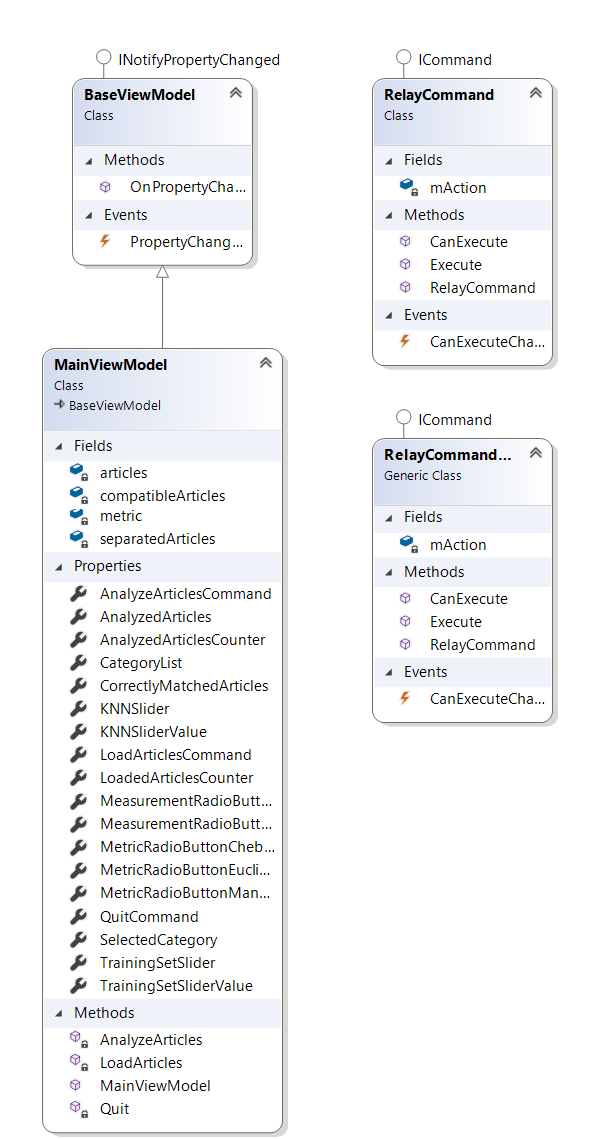
\includegraphics[width=1\textwidth]{{Rysunki/DiagramLogic.png}}
	\caption{Diagram UML wygenerowany dla projektu Logic}
\end{figure}

\subsection{ViewModel}
Projekt ViewModel ma za zadanie odseparować logikę programu od interfejsu graficznego. \newline

Klasa MainViewModel przyjmuje dane wejściowe od użytkownika i reaguje na jego poczynania wywołując wybrane akcje z logiki programu oraz odpowiada za odświeżanie widoków w interfejsie graficznym.

\begin{figure}[H]
	\centering
	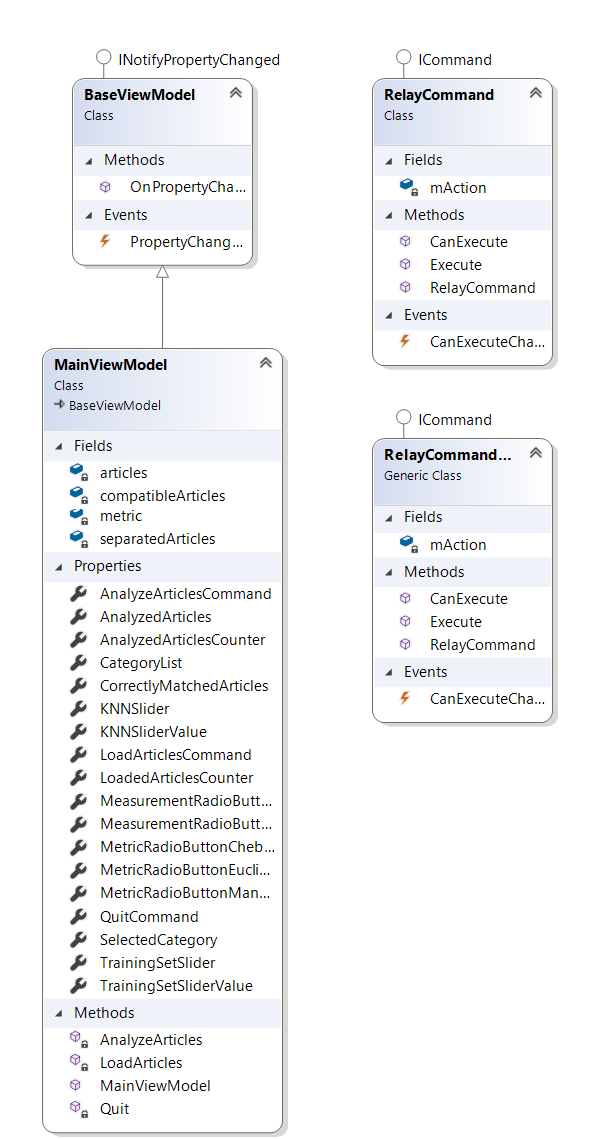
\includegraphics[width=0.9\textwidth]{{Rysunki/DiagramViewModel.png}}
	\caption{Diagram UML wygenerowany dla projektu MainViewModel}
\end{figure}

\subsection{GUI}
Projekt GUI (graphical user interface) implementuje przejrzysty oraz łatwy w obsłudze graficzny interfejs użytkownika. 

\begin{figure}[H]
	\centering
	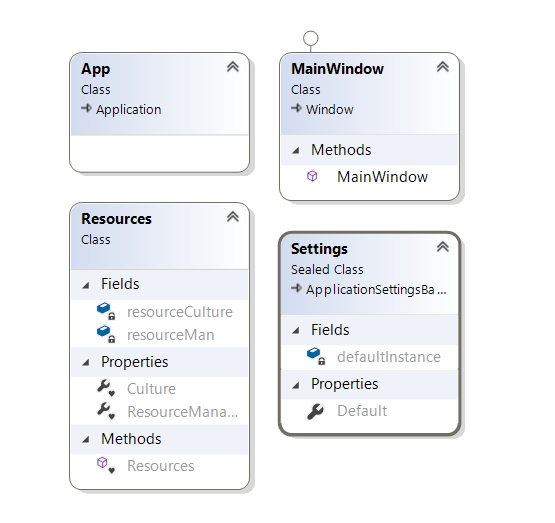
\includegraphics[width=1\textwidth]{{Rysunki/DiagramGUI.png}}
	\caption{Diagram UML wygenerowany dla projektu GUI}
\end{figure}

\section{Materiały i metody}

Klasyfikacja dotycząca lokalizacji przeprowadzana była jedynie na danych, których pole places przyjmowało jedną z wartości: west-germany, usa, france, uk, canada, japan. \newline

Klasyfikacja dotycząca tematów przeprowadzana była jedynie na danych, które pole topics przyjmowało jedną z wartości: gold, cocoa, sugar, coffe, grain. \newline

Danymi jakie sami przygotowaliśmy do analizy były teksty piosenek znanych artystów. Posiadały one jedną kategorię - author. Przyjmowało ono jedną z wartości: taylor swift, macklemore, twenty one pilots, eminem, ed sheeran, black eyed peas.

\subsection{Wpływ liczby k sąsiadów oraz wyboru metryki na klasyfikację}

Klasyfikacja tekstów została wykonana wszystkimi dostępnymi metodami ekstrakcji cech dla wszystkich trzech metryk. Dla każdego przypadku testowego dokonano klasyfikacji tekstu dla k $\in$ \{2, 3, 5, 7, 10, 15, 20\} najbliższych sąsiadów. Zbiór treningowy stanowił zawsze 60\% artykułów, zaś zbiór testowy 40\% artykułów. \newline

\subsection{Wpływ podziału tekstów na zbiory treningowe i testowe na klasyfikację}

Klasyfikacja tekstów została wykonana przy pomocy Term frequency oraz własnych charakterystyk dla metryki Euklidesowej. Dla każdego przypadku testowego dokonano klasyfikacji tekstu dla najodpowiedniejszych k dla danego sposobu ekstrakcji cech oraz metryki. Zbiór treningowy w kolejnych próbach stanowił, 80\% 60\% oraz 40\% artykułów. \newline

\subsection{Wpływ konkretnych cech na klasyfikację}
Klasyfikacja tekstów została wykonana przy pomocy ekstrakcji cech charakterystycznych dla metryki \_ oraz dla zbioru treningowego stanowiącego \_ artykułów.

\section{Wyniki}

Poniższej umieszczone tabele oraz wykresy są wynikami przeprowadzonych przez nas eksperymentów.

\subsection{Wpływ liczby k sąsiadów oraz wyboru metryki na klasyfikację}

\begin{table}[H]
	\centering
	\begin{tabular}{c c c c} 
		\hline
		\textbf{k} & \textbf{places [\%]} & \textbf{topics [\%]} &  \textbf{authors [\%]} \\ [0.5ex] 
		\hline
		\hline 
		2 & 74.4 & 53.7 & 43.9 \\ 
		3 & 78.5 & 52.2 & 43.9 \\
		5 & 80.2 & 52.2 & 36.6 \\
		7 & 81.0 & 53.7 & 26.8 \\
		10 & 81.5 & 60.4 & 24.4 \\
		15 & 81.6 & 62.7 & 29.3 \\
		20 & 81.4 & 61.2 & 31.7 \\ 
		\hline
	\end{tabular}
	\caption{Skuteczność klasyfikacji dla metryki Euklidesowej dla pierwszego sposobu ekstrakcji}
\end{table}

\begin{table}[H]
	\centering
	\begin{tabular}{c c c c} 
		\hline
		\textbf{k} & \textbf{places [\%]} & \textbf{topics [\%]} &  \textbf{authors [\%]} \\ [0.5ex] 
		\hline
		\hline 
		2 & 75.4 & 56.7 & 36.6 \\ 
		3 & 79.4 & 56.7 & 39.0 \\
		5 & 81.0 & 61.2 & 36.6 \\
		7 & 81.3 & 59.0 & 31.7 \\
		10 & 81.9 & 64.9 & 24.4 \\
		15 & 82.0 & 64.9 & 29.3 \\
		20 & 82.1 & 63.4 & 29.3 \\ 
		\hline
	\end{tabular}
	\caption{Skuteczność klasyfikacji dla metryki ulicznej dla pierwszego sposobu ekstrakcji}
\end{table}

\begin{table}[H]
	\centering
	\begin{tabular}{c c c c} 
		\hline
		\textbf{k} & \textbf{places [\%]} & \textbf{topics [\%]} &  \textbf{authors [\%]} \\ [0.5ex] 
		\hline
		\hline 
		2 & 80.3 & 14.9 & 17.1 \\ 
		3 & 80.3 & 44.0 & 17.1 \\
		5 & 80.3 & 44.0 & 17.1 \\
		7 & 80.3 & 44.0 & 17.1 \\
		10 & 80.3 & 44.0 & 17.1 \\
		15 & 80.3 & 44.0 & 17.1 \\
		20 & 80.3 & 44.0 & 17.1 \\ 
		\hline
	\end{tabular}
	\caption{Skuteczność klasyfikacji dla metryki Czebyszewa dla pierwszego sposobu ekstrakcji}
\end{table}

\begin{figure}[H]
	\centering
	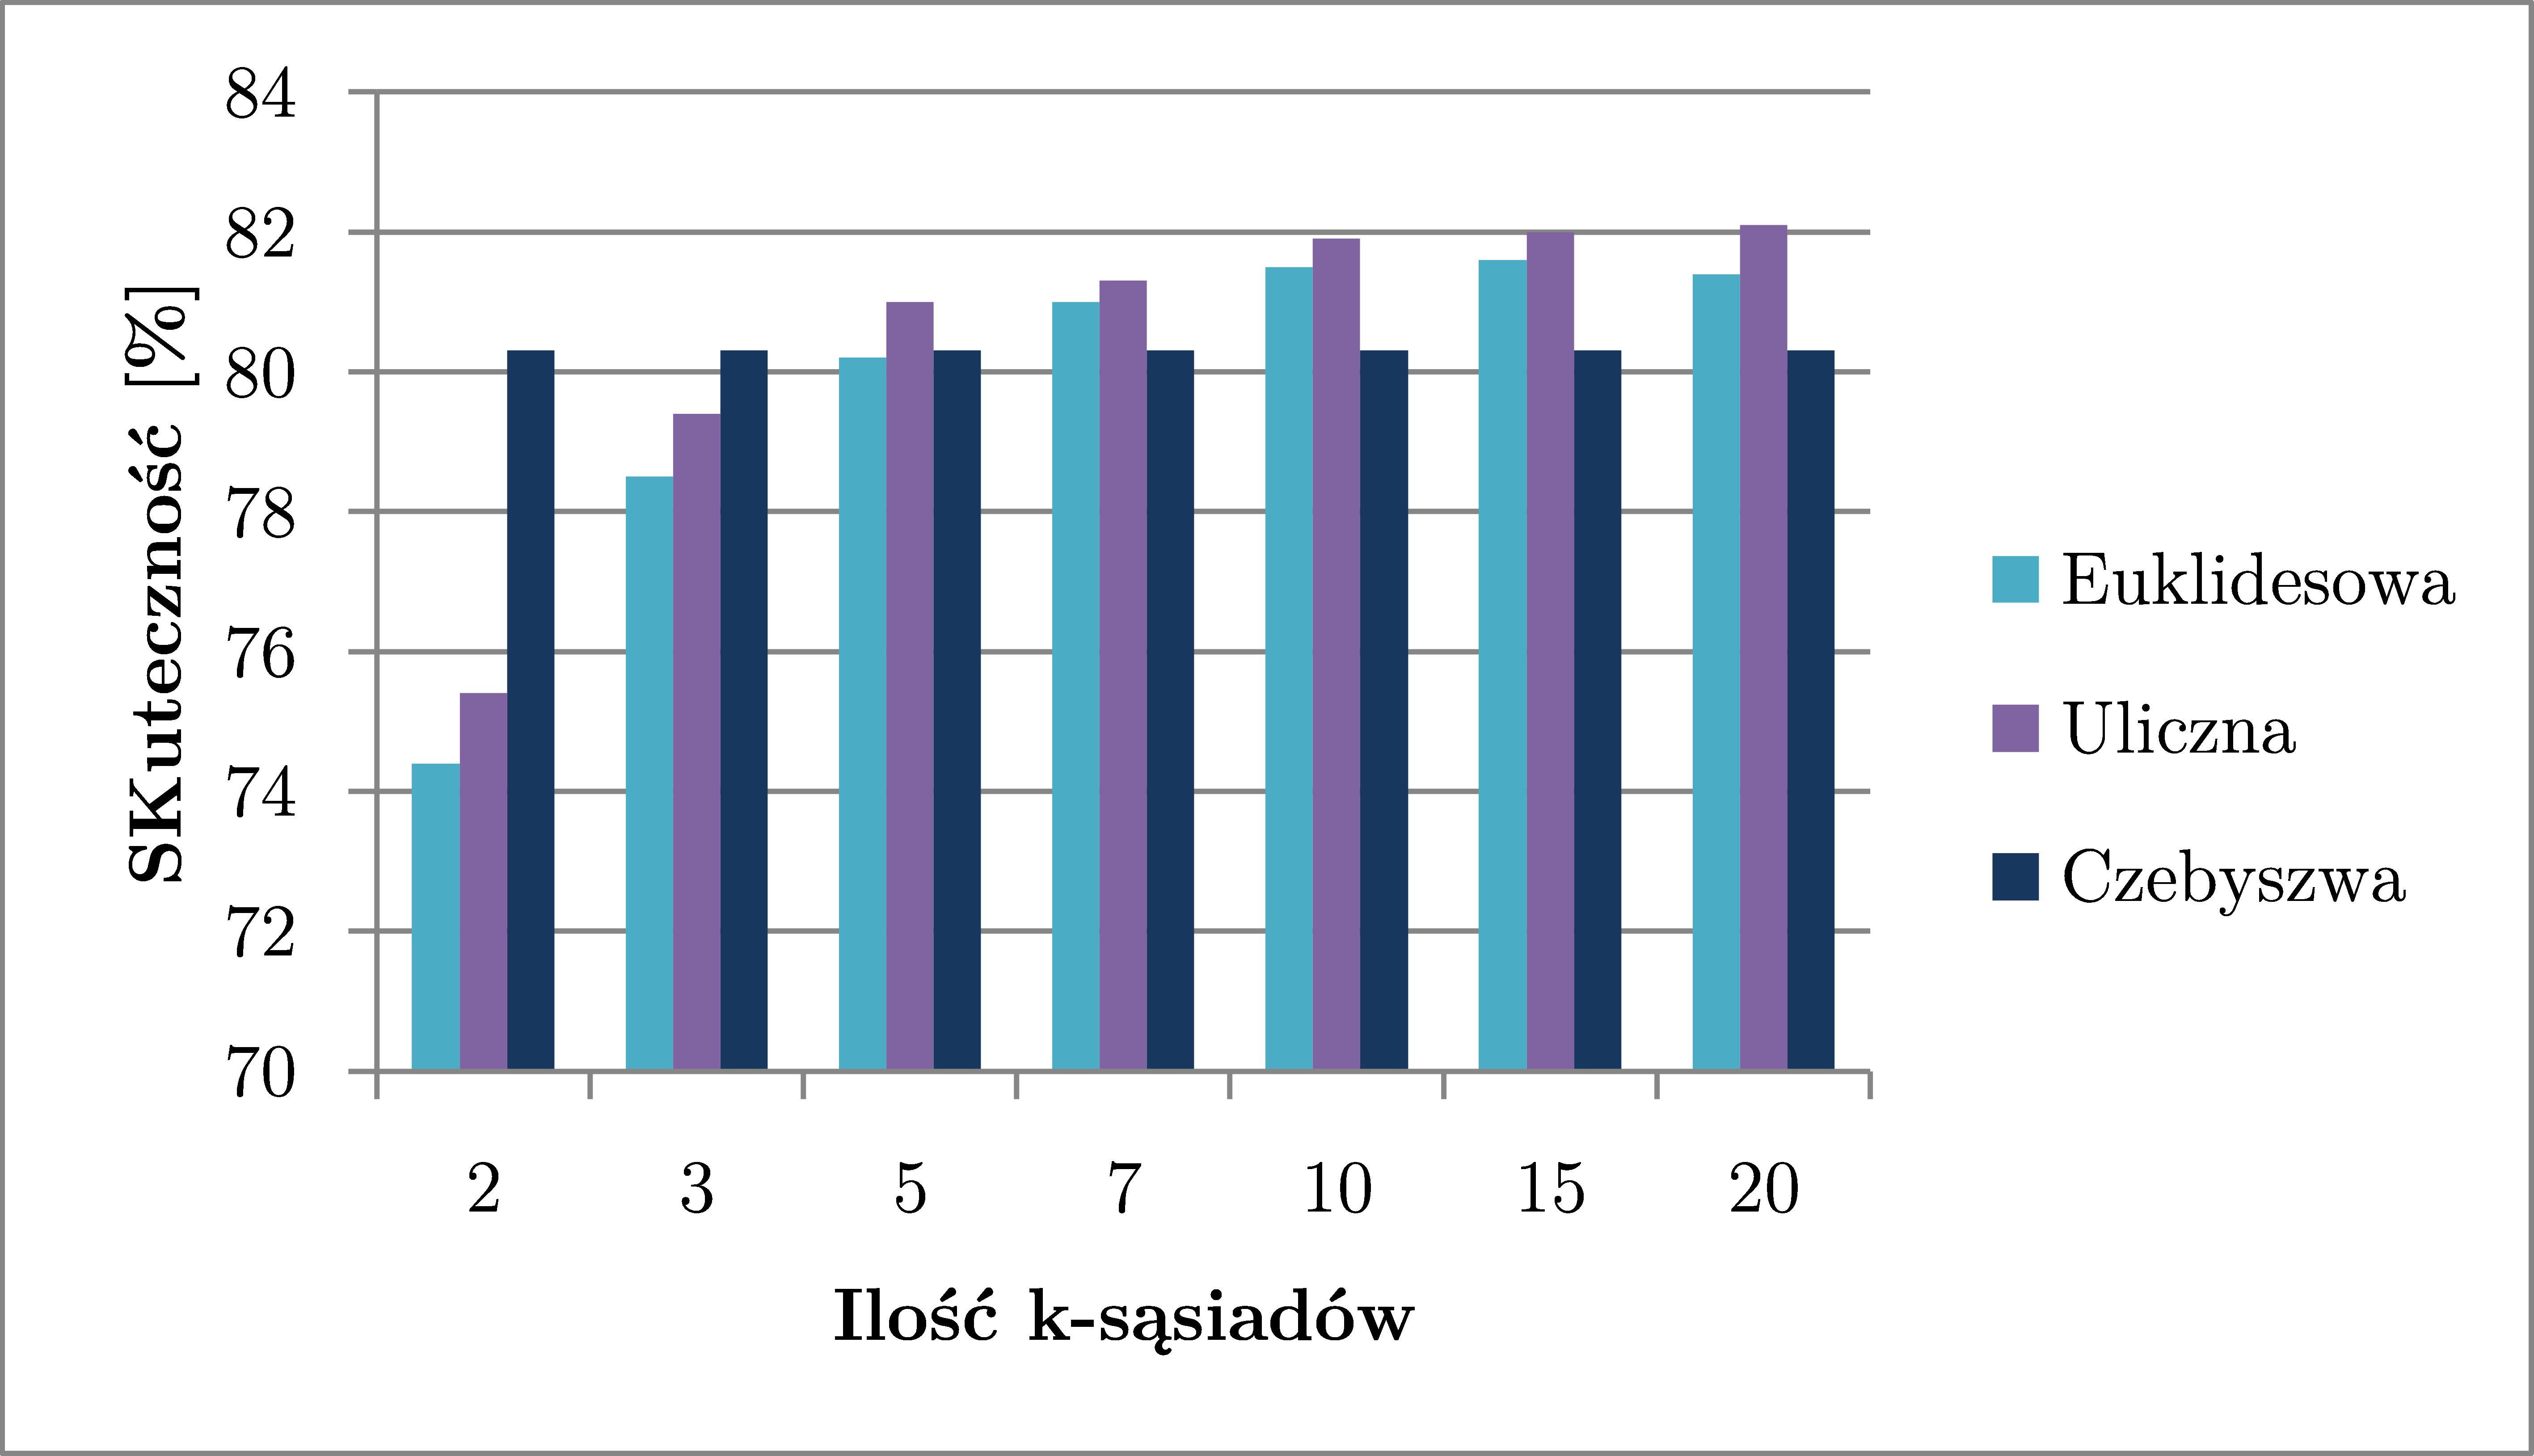
\includegraphics[width=0.9\textwidth]{{Rysunki/TF-places.png}}
	\caption{Dane z Tabel 1-3 dla kategorii places}
\end{figure}

\begin{figure}[H]
	\centering
	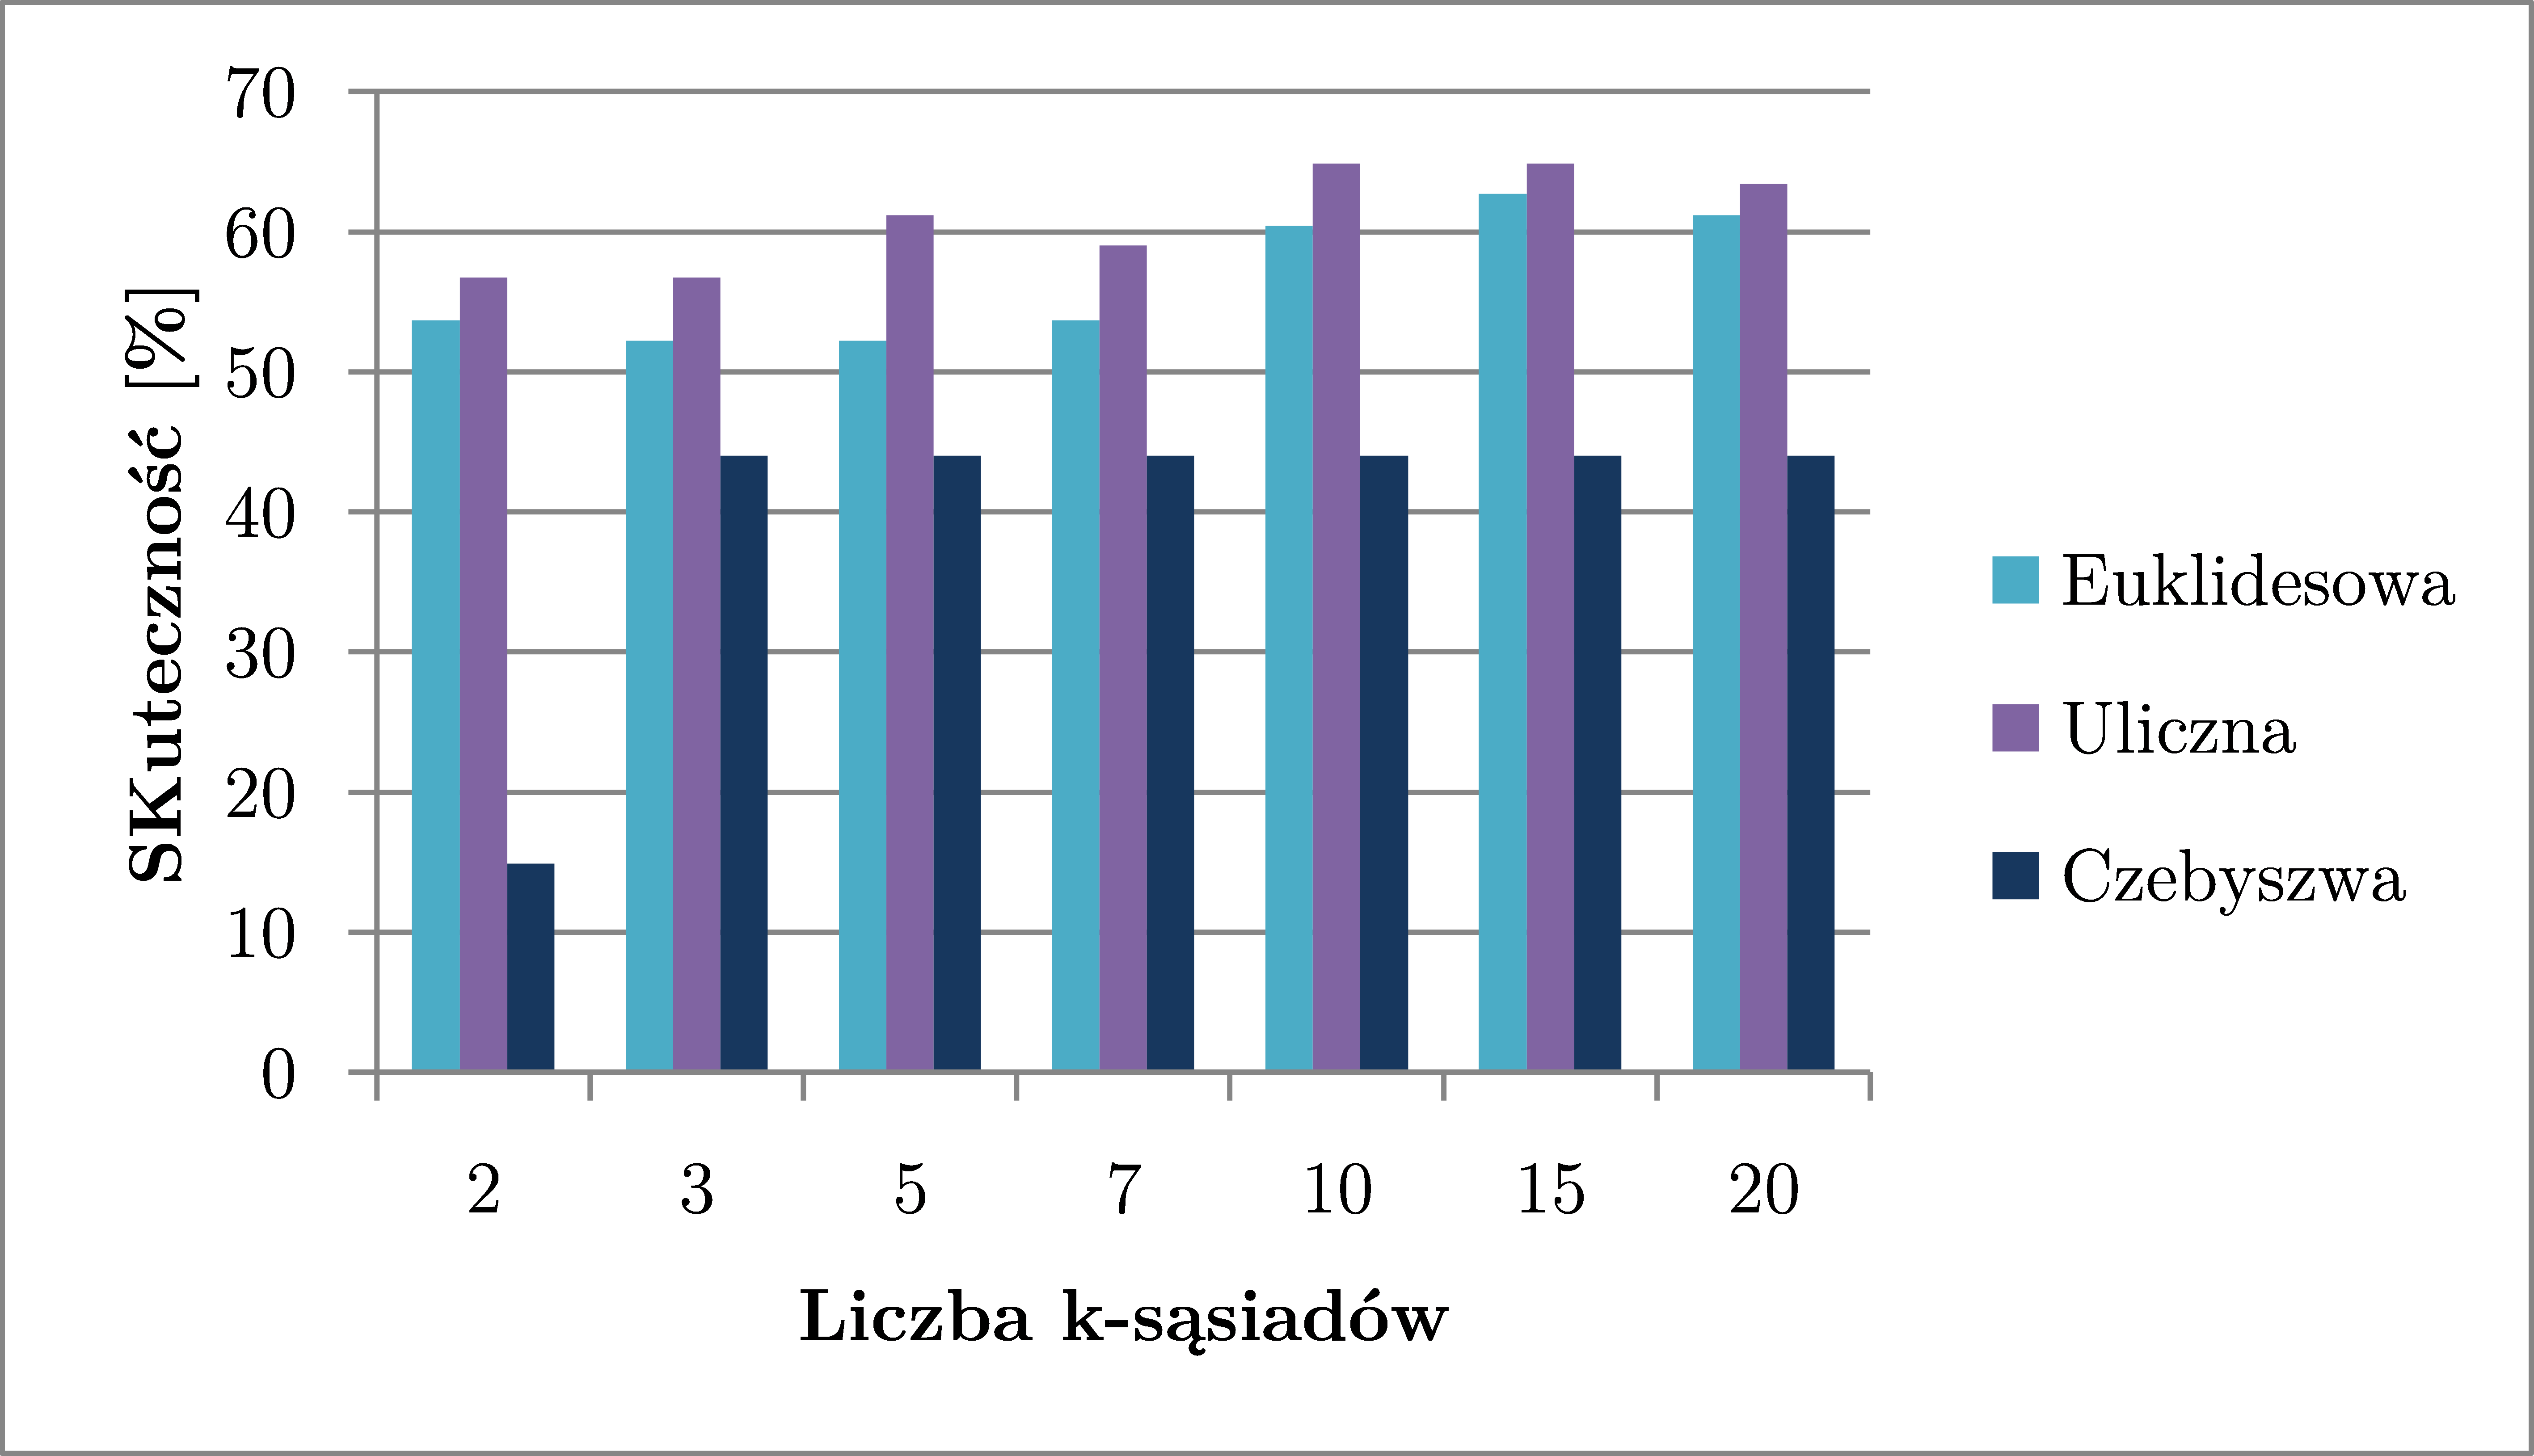
\includegraphics[width=0.9\textwidth]{{Rysunki/TF-topics.png}}
	\caption{Dane z Tabel 1-3 dla kategorii topics}
\end{figure}

\begin{figure}[H]
	\centering
	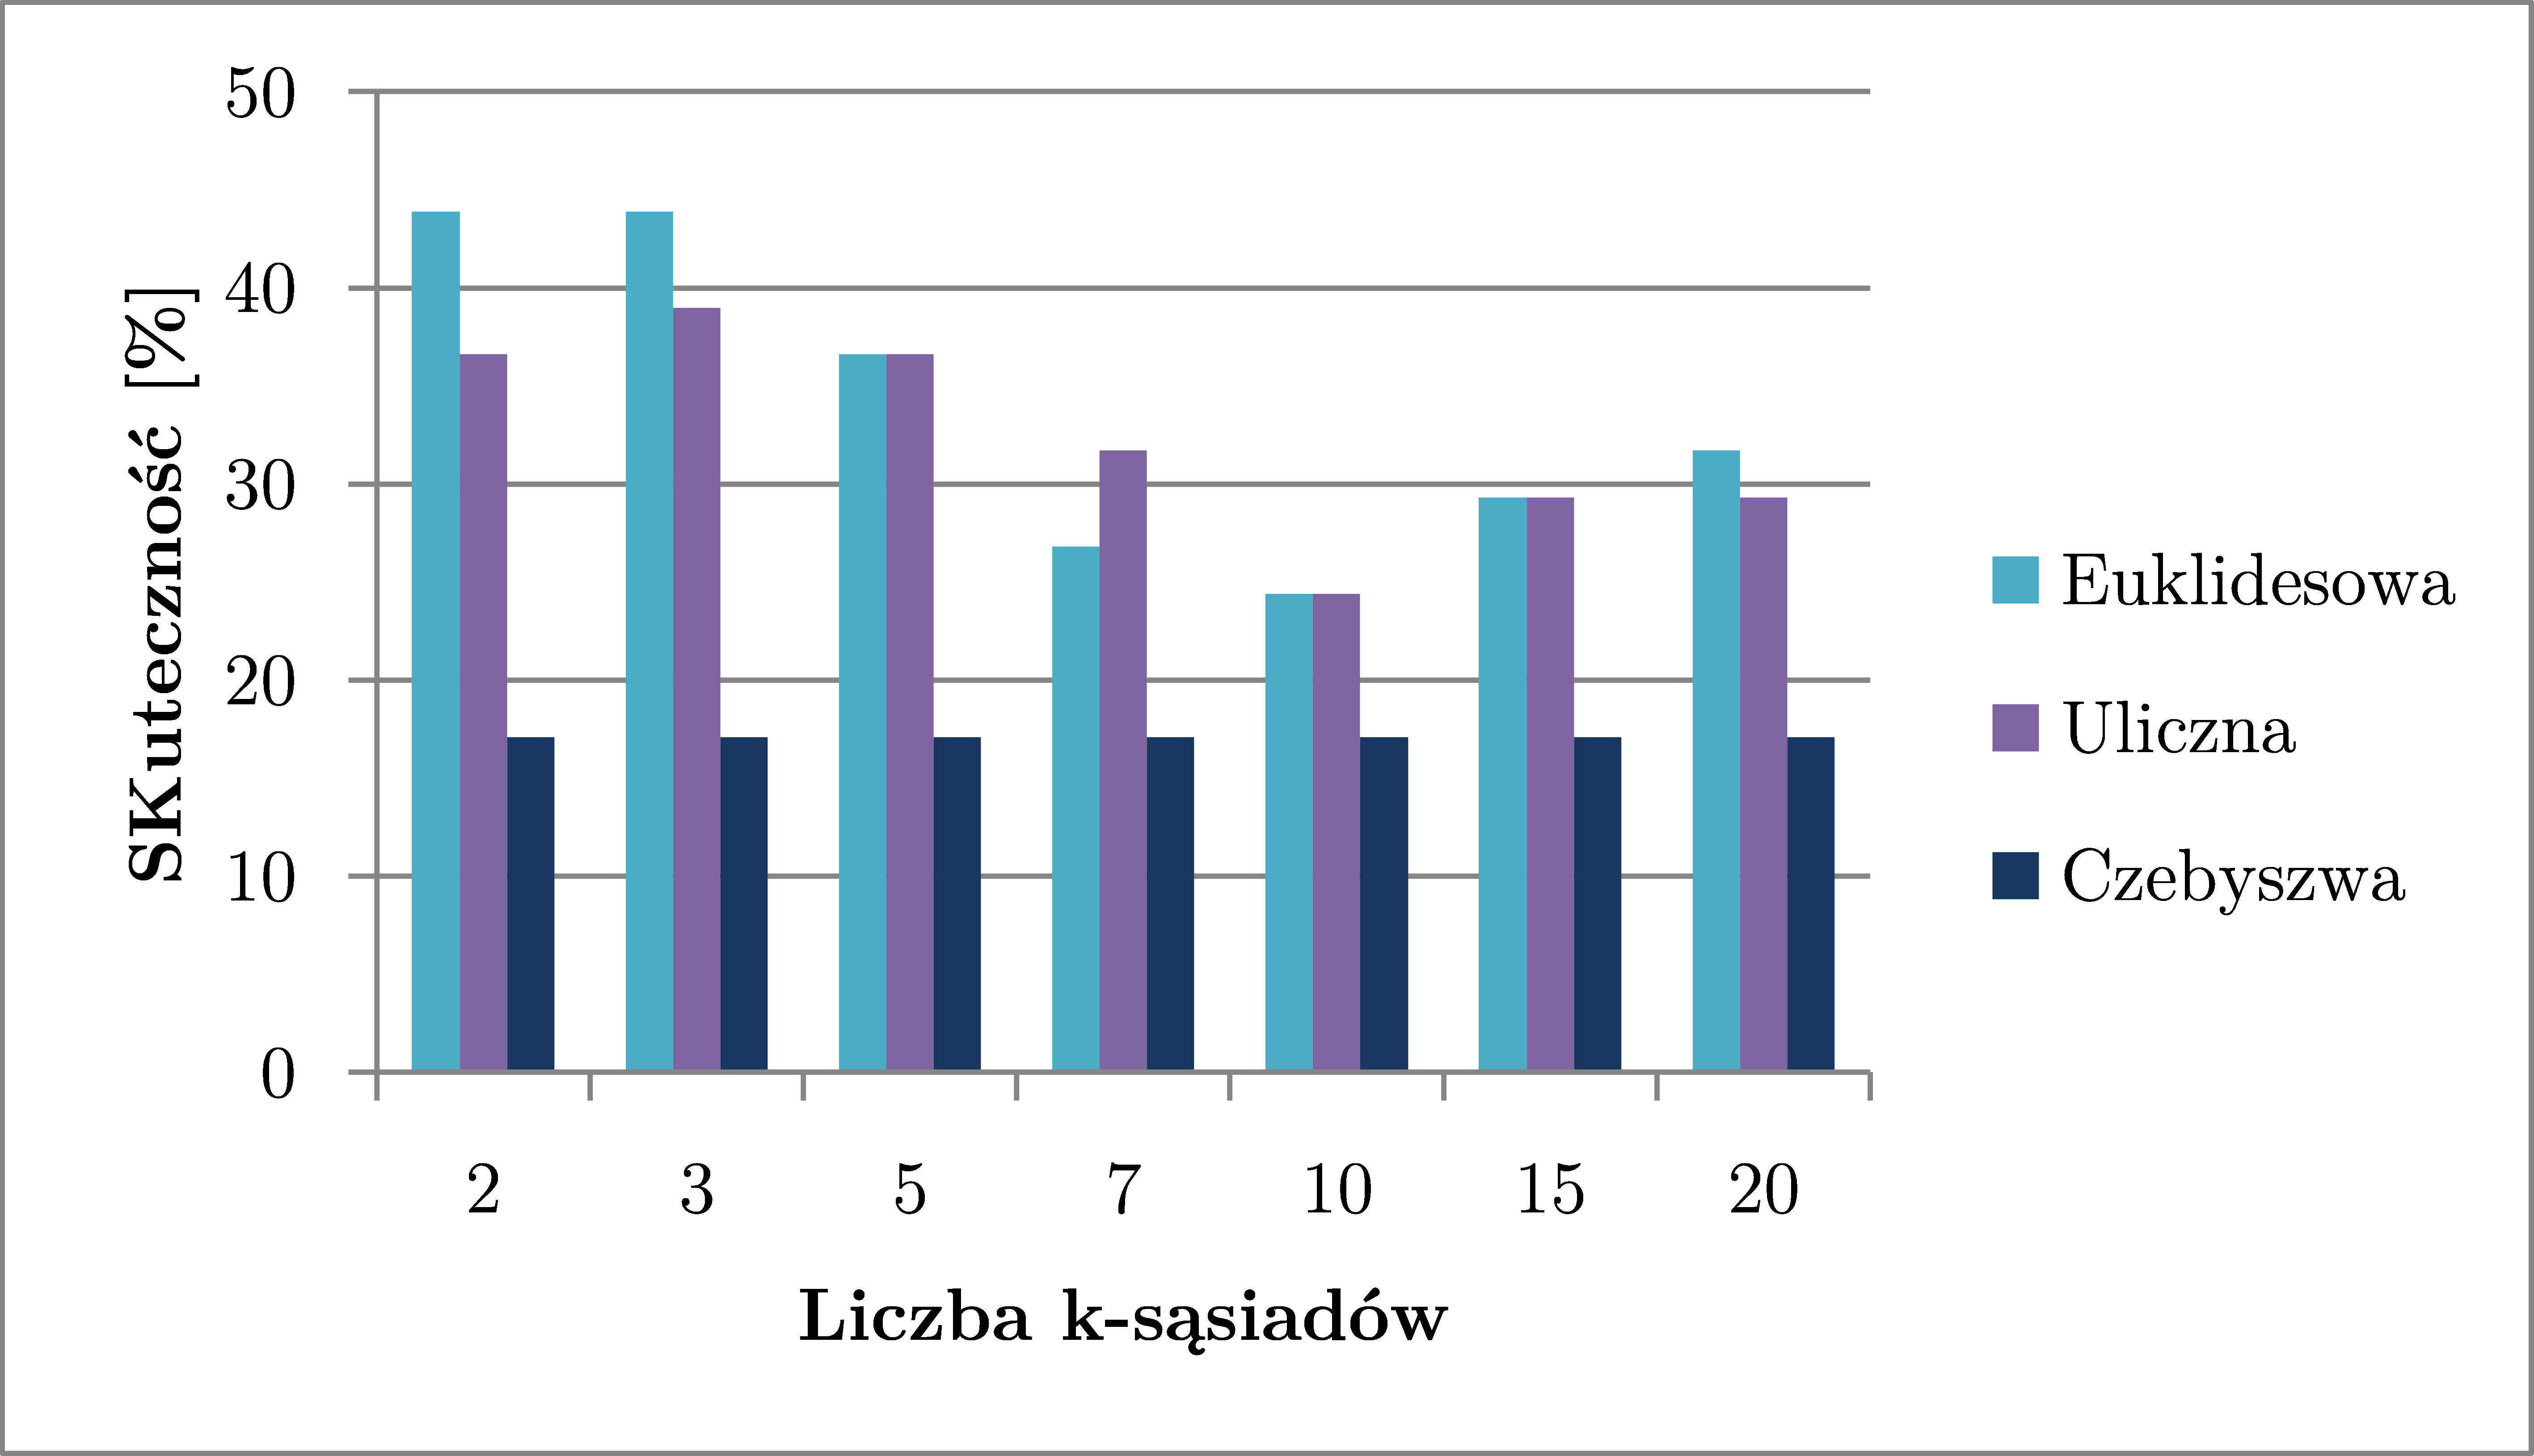
\includegraphics[width=0.9\textwidth]{{Rysunki/TF-authors.png}}
	\caption{Dane z Tabel 1-3 dla kategorii authors (własne teksty)}
\end{figure}

\begin{table}[H]
	\centering
	\begin{tabular}{c c c c} 
		\hline
		\textbf{k} & \textbf{places [\%]} & \textbf{topics [\%]} &  \textbf{authors [\%]} \\ [0.5ex] 
		\hline
		\hline 
		2 & 79.0 & 63.4 & 22.0 \\ 
		3 & 82.0 & 64.2 & 19.5 \\
		5 & 82.1 & 59.0 & 29.3 \\
		7 & 83.3 & 62.1 & 22.0 \\
		10 & 82.0 & 64.9 & 26.8 \\
		15 & 81.9 & 67.9 & 24.4 \\
		20 & 81.1 & 67.1 & 17.1 \\ 
		\hline
	\end{tabular}
	\caption{Skuteczność klasyfikacji dla metryki Euklidesowej dla drugiego sposobu ekstrakcji}
\end{table}

\begin{table}[H]
	\centering
	\begin{tabular}{c c c c} 
		\hline
		\textbf{k} & \textbf{places [\%]} & \textbf{topics [\%]} &  \textbf{authors [\%]} \\ [0.5ex] 
		\hline
		\hline 
		2 & 80.2 & 59.7 & 22.0 \\ 
		3 & 82.4 & 65.7 & 19.5 \\
		5 & 82.6 & 67.2 & 29.3 \\
		7 & 83.3 & 67.2 & 22.0 \\
		10 & 82.6 & 67.2 & 26.8 \\
		15 & 82.1 & 67.2 & 24.4 \\
		20 & 81.6 & 67.9 & 17.1 \\ 
		\hline
	\end{tabular}
	\caption{Skuteczność klasyfikacji dla metryki ulicznej dla drugiego sposobu ekstrakcji}
\end{table}

\begin{table}[H]
	\centering
	\begin{tabular}{c c c c} 
		\hline
		\textbf{k} & \textbf{places [\%]} & \textbf{topics [\%]} &  \textbf{authors [\%]} \\ [0.5ex] 
		\hline
		\hline 
		2 & 77.0 & 14.9 & 17.1 \\ 
		3 & 77.0 & 44.0 & 17.1 \\
		5 & 77.0 & 44.0 & 17.1 \\
		7 & 77.0 & 44.0 & 17.1 \\
		10 & 77.0 & 44.0 & 17.1 \\
		15 & 77.0 & 44.0 & 17.1 \\
		20 & 77.0 & 44.0 & 17.1 \\ 
		\hline
	\end{tabular}
	\caption{Skuteczność klasyfikacji dla metryki Czebyszewa dla drugiego sposobu ekstrakcji}
\end{table}

\begin{figure}[H]
	\centering
	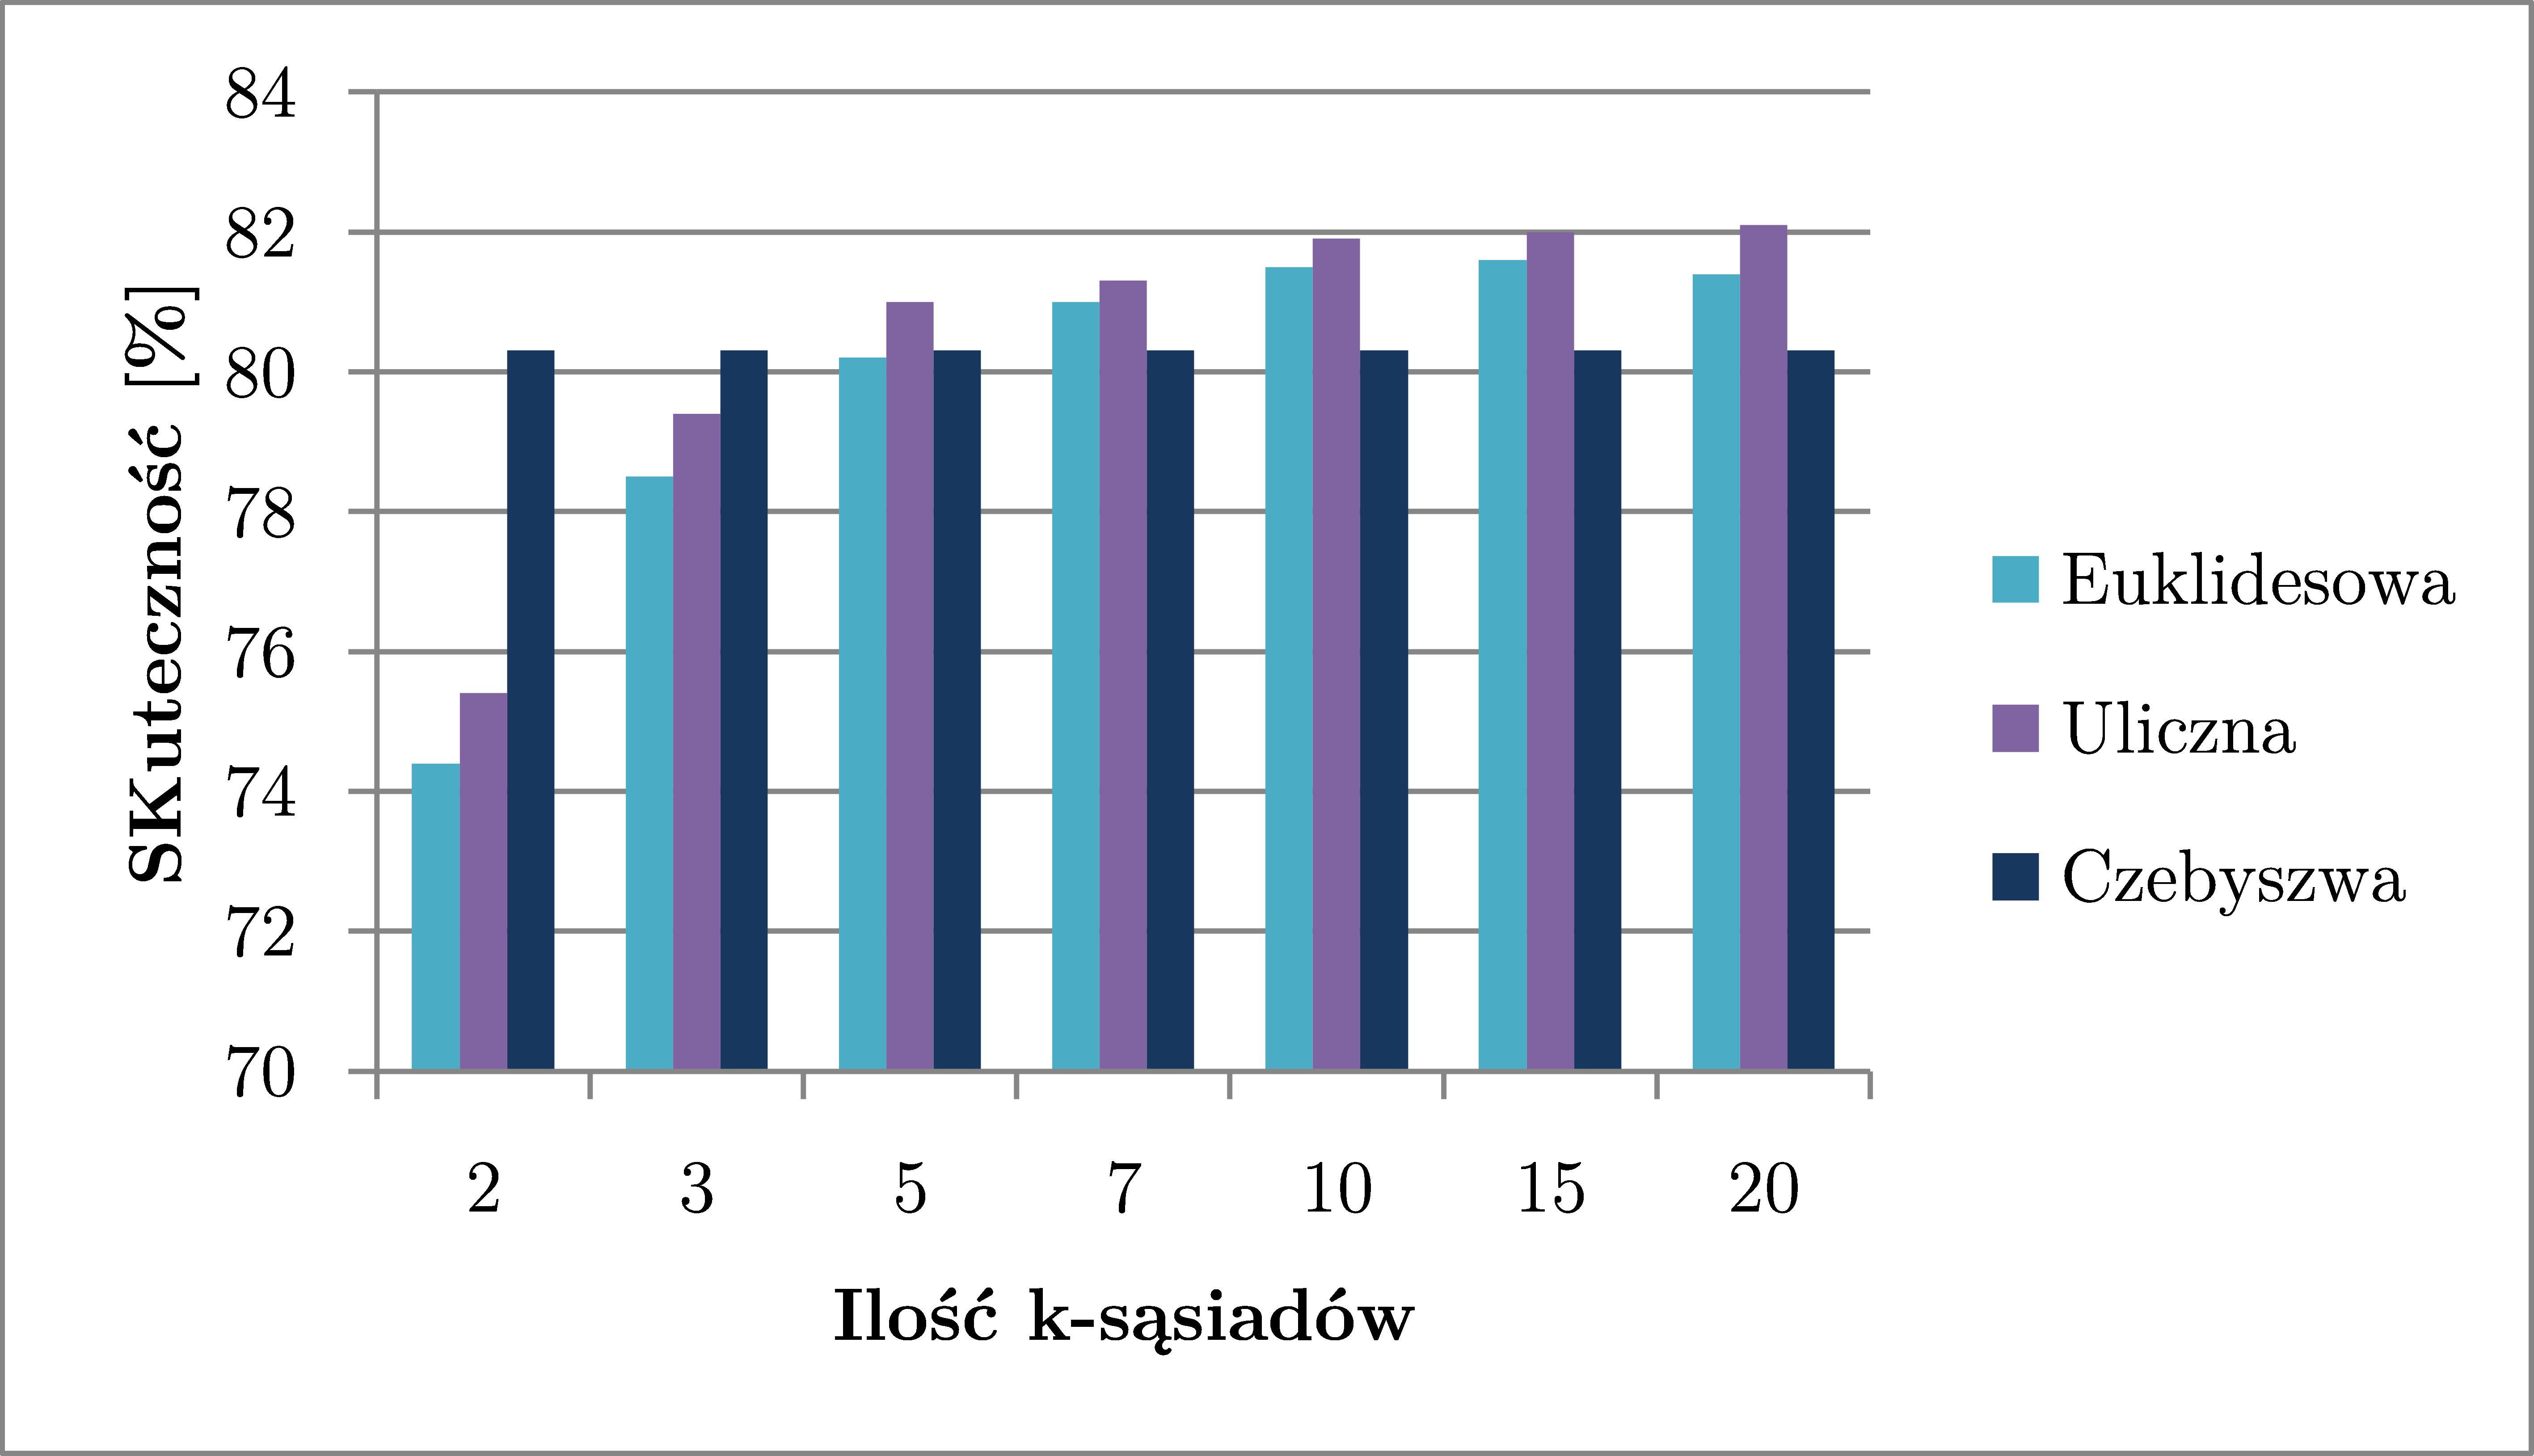
\includegraphics[width=0.9\textwidth]{{Rysunki/TF-places.png}}
	\caption{Dane z Tabel 4-6 dla kategorii places}
\end{figure}

\begin{figure}[H]
	\centering
	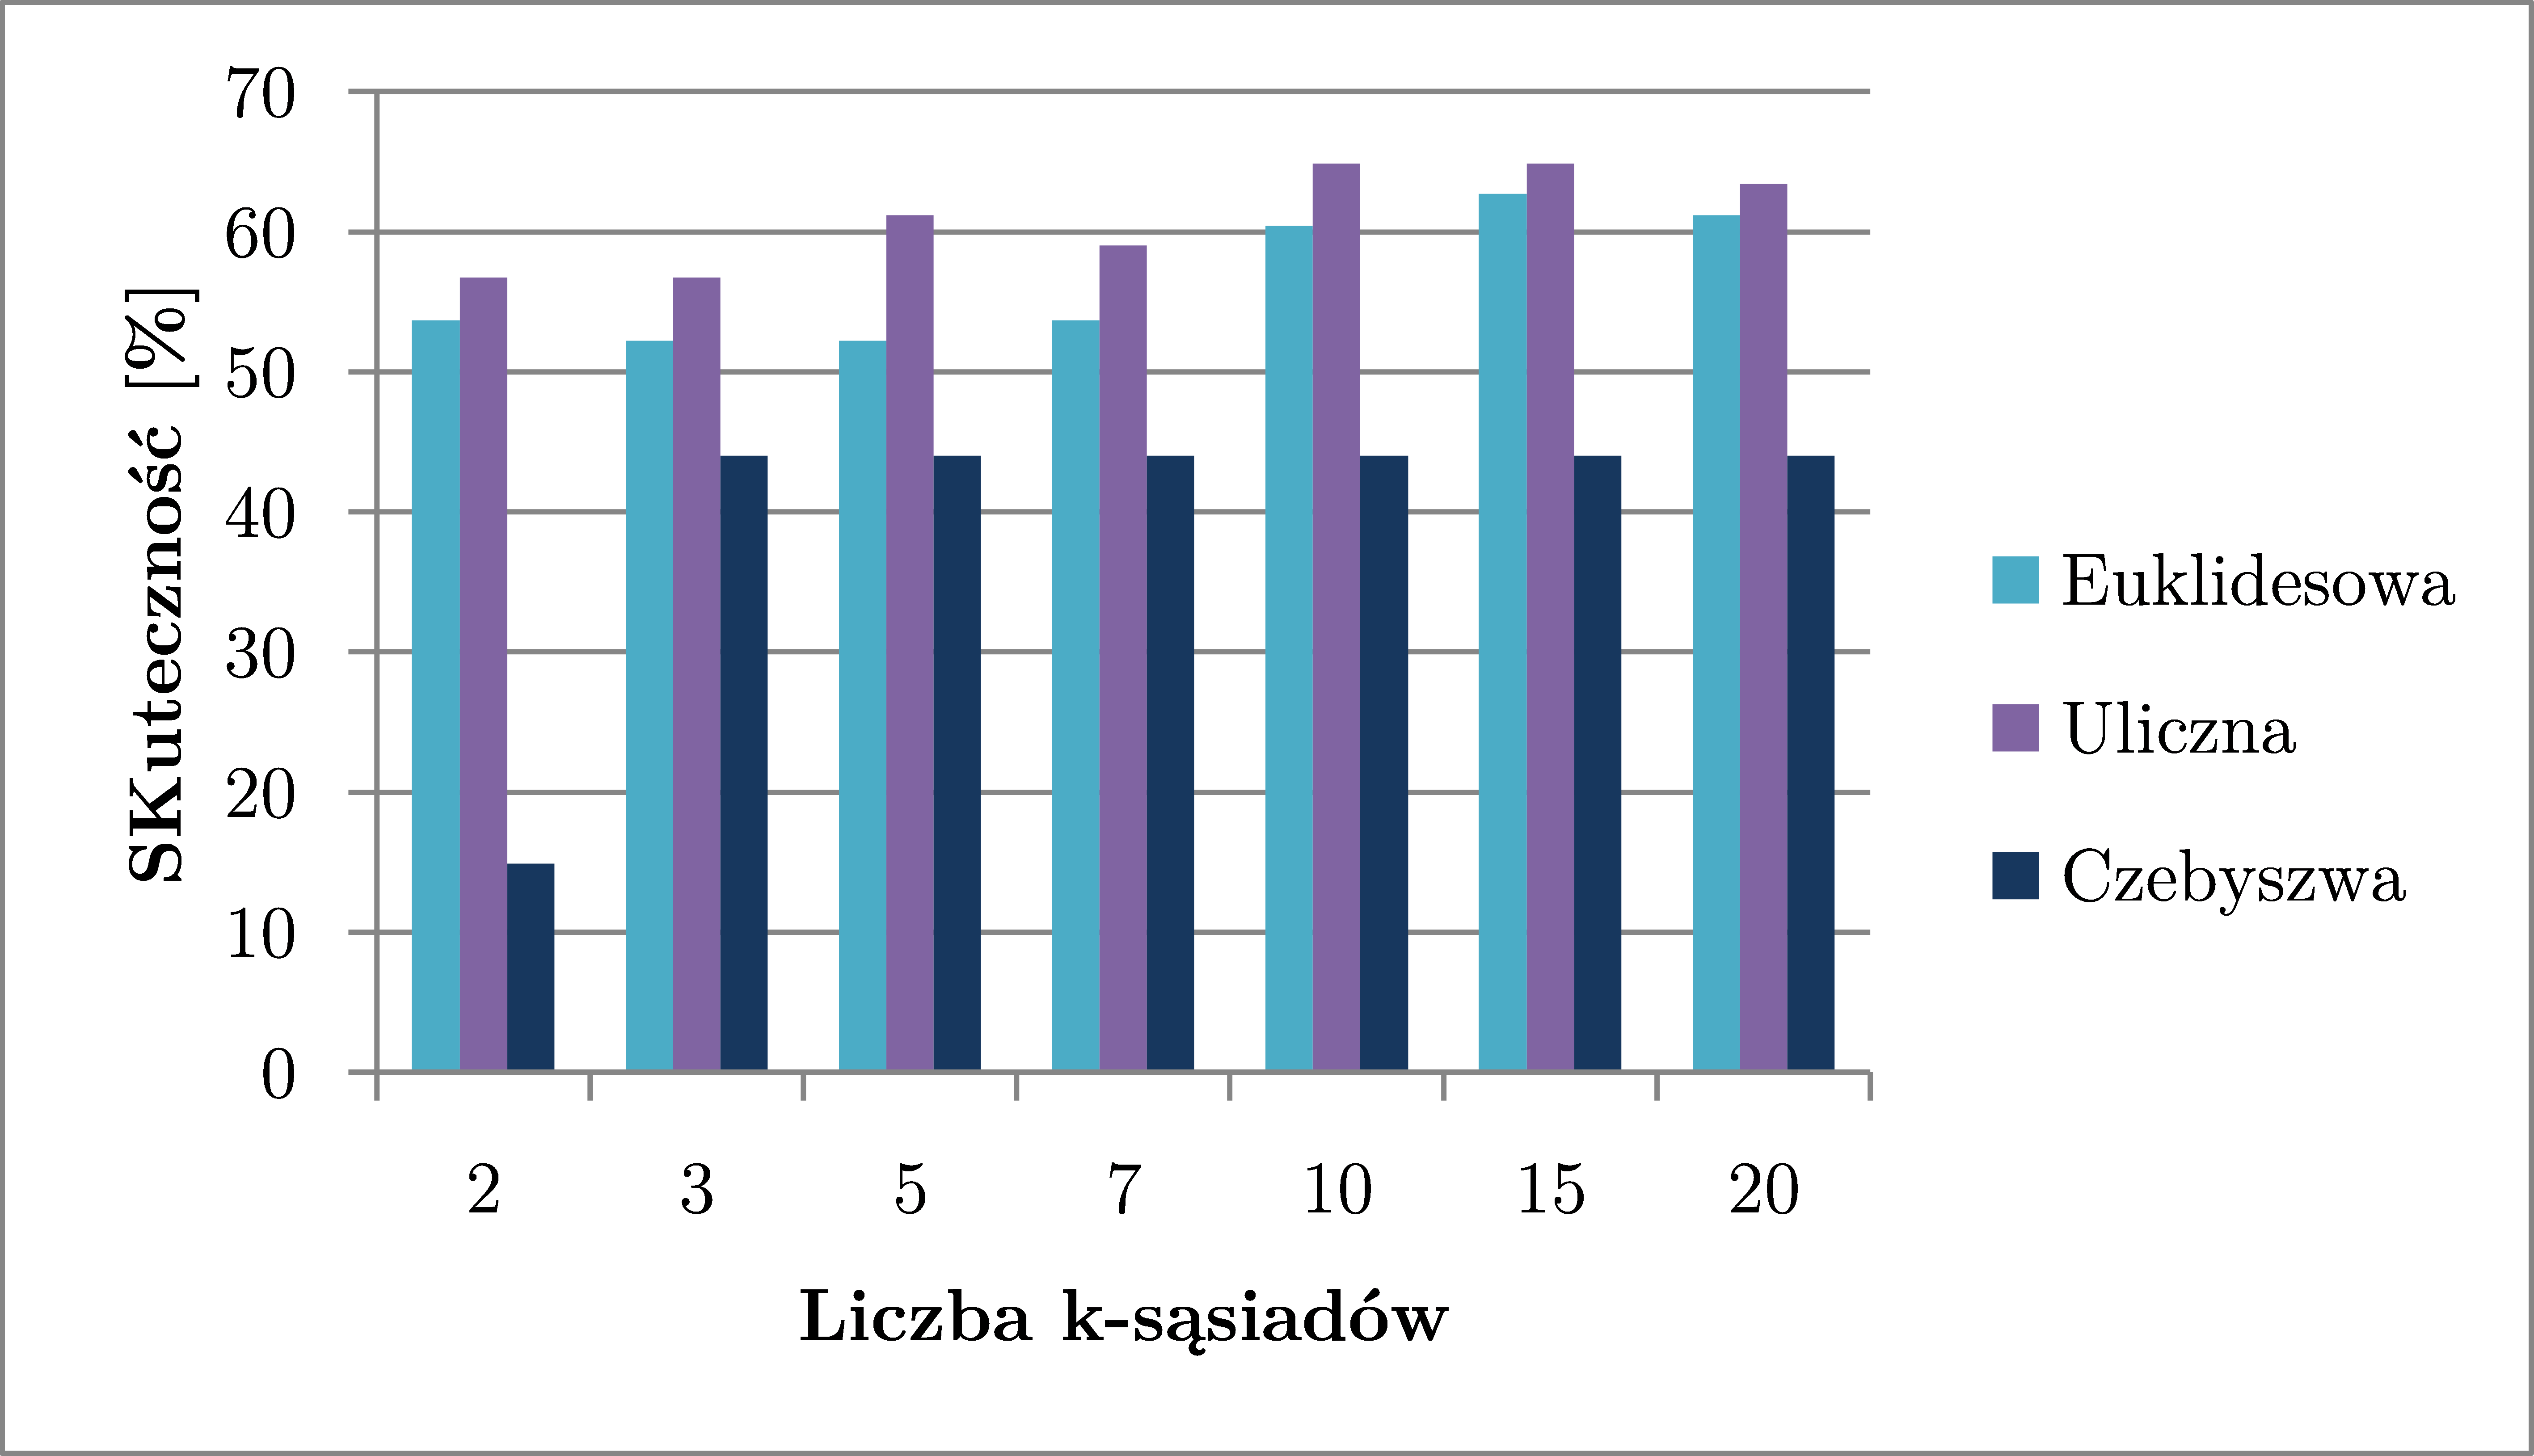
\includegraphics[width=0.9\textwidth]{{Rysunki/TF-topics.png}}
	\caption{Dane z Tabel 4-6 dla kategorii topics}
\end{figure}

\begin{figure}[H]
	\centering
	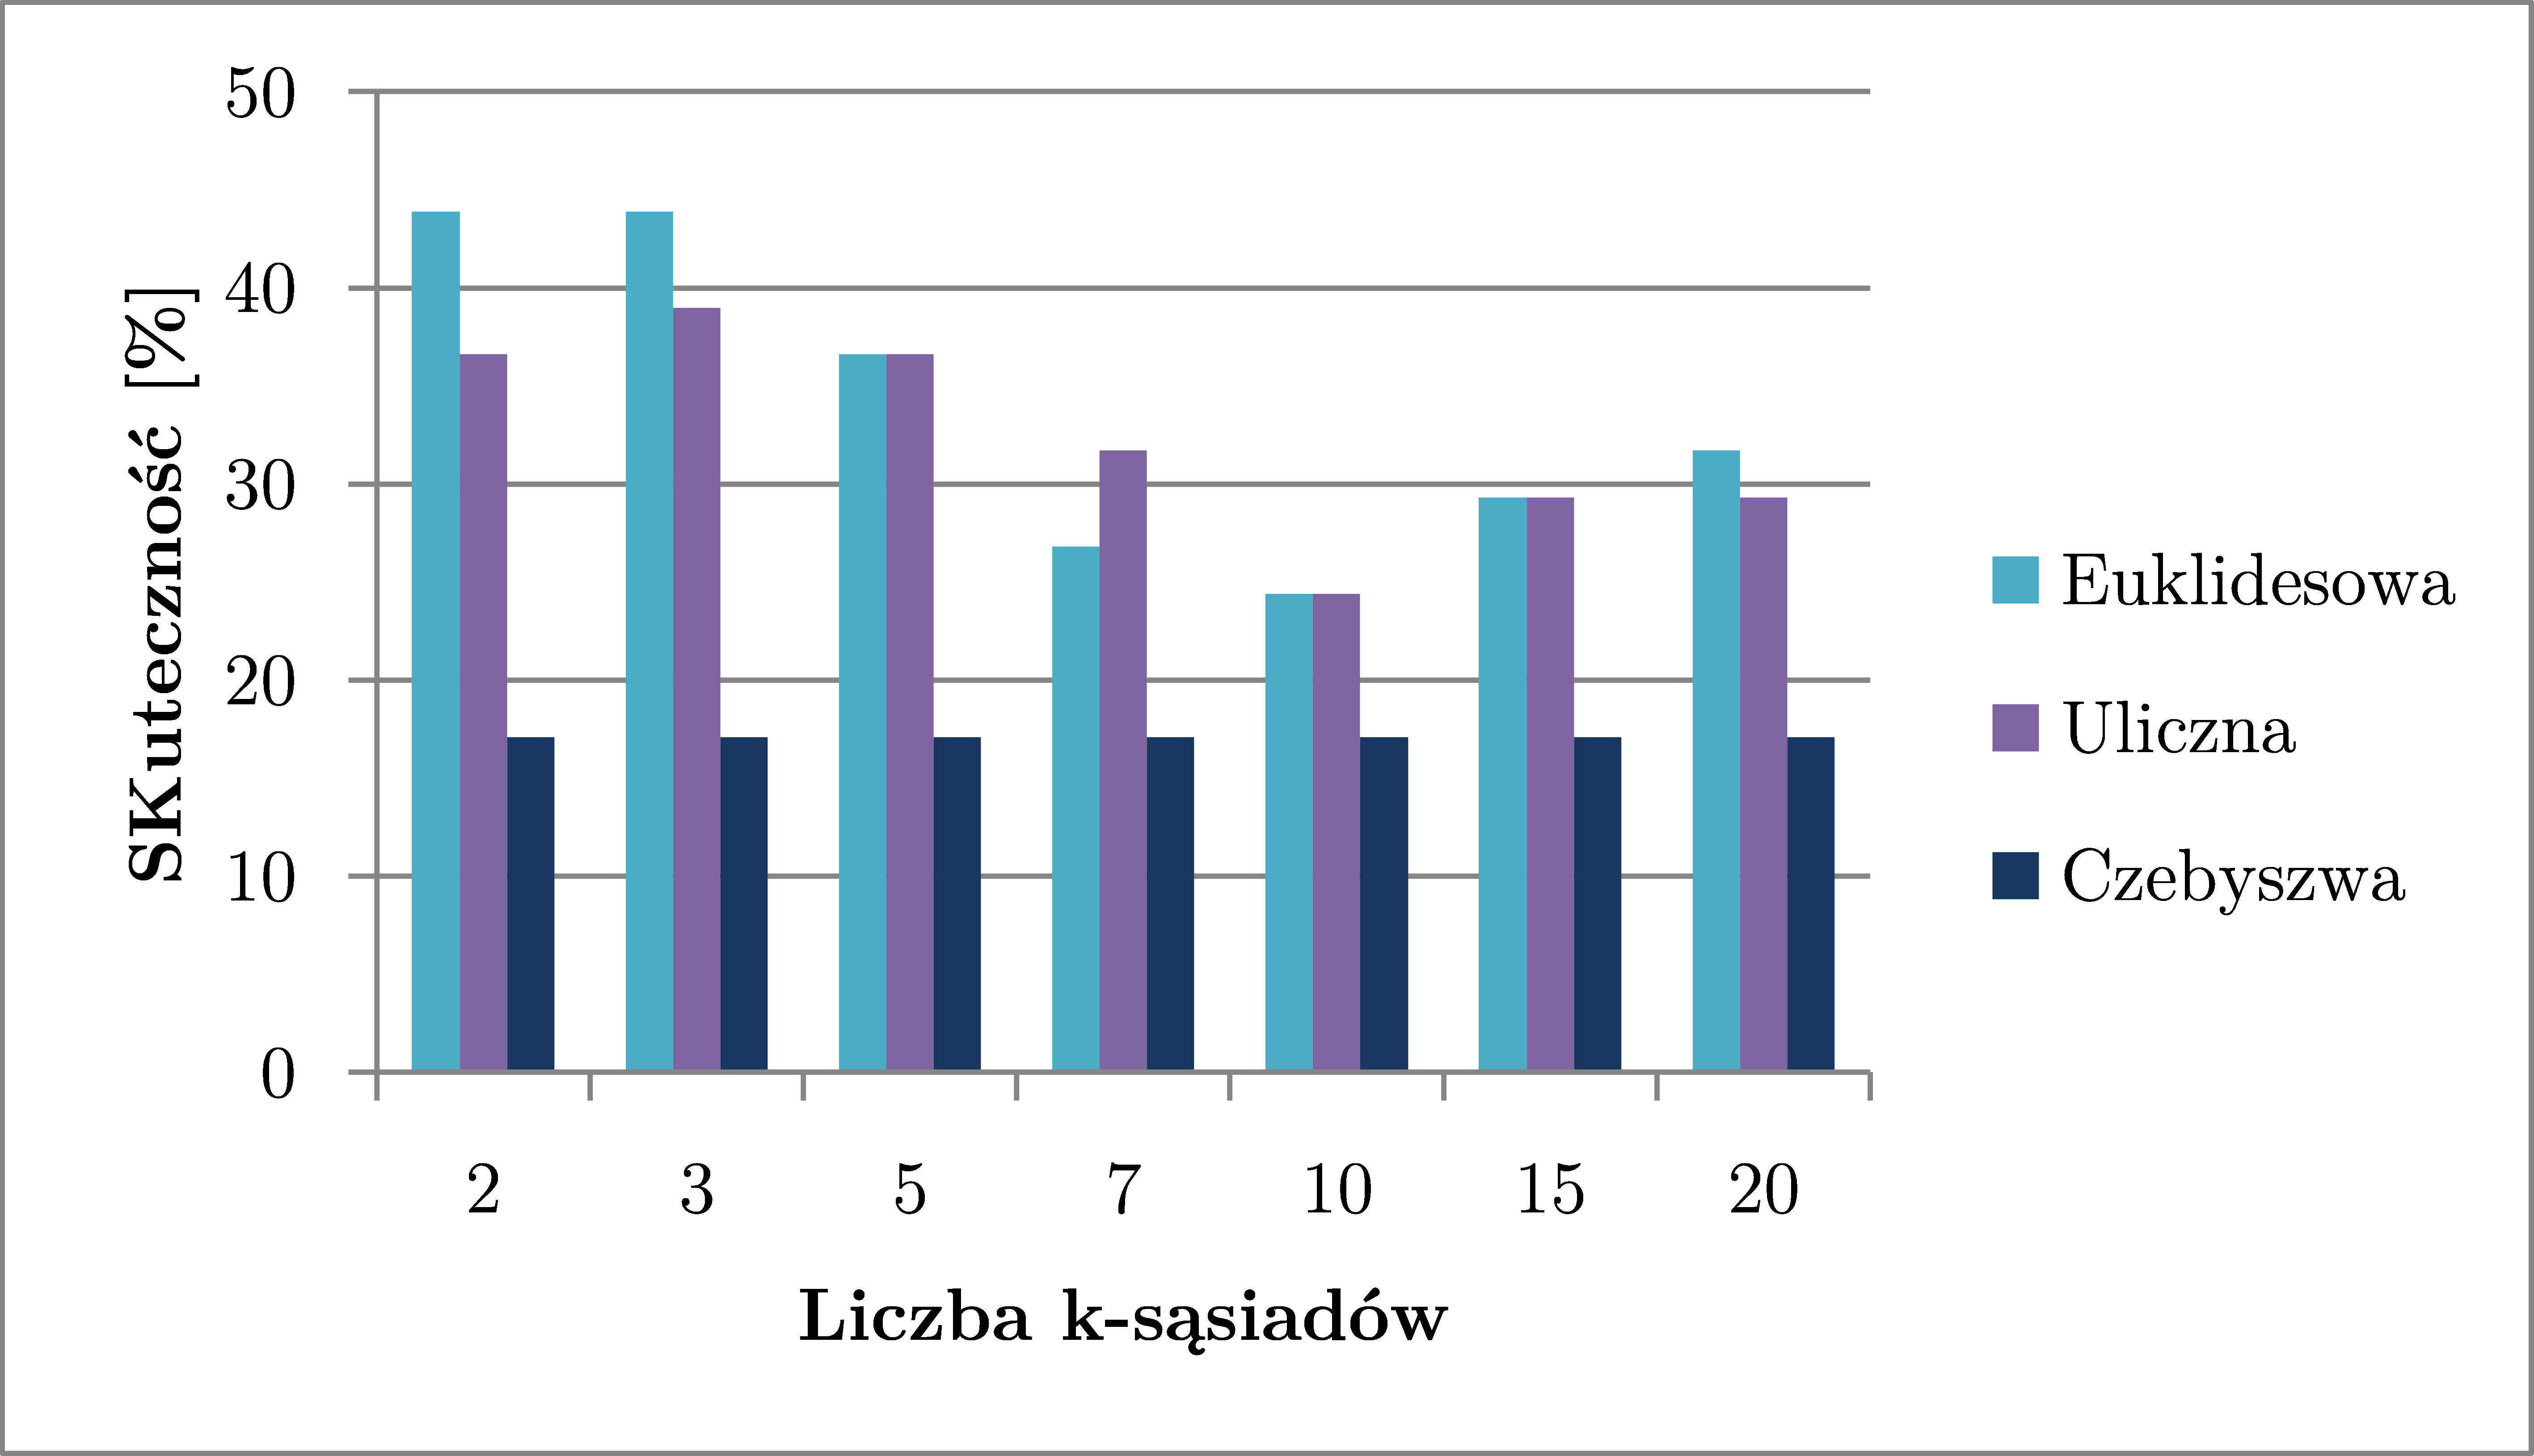
\includegraphics[width=0.9\textwidth]{{Rysunki/TF-authors.png}}
	\caption{Dane z Tabel 4-6 dla kategorii authors (własne teksty)}
\end{figure}

\begin{table}[H]
	\centering
	\begin{tabular}{c c c c} 
		\hline
		\textbf{k} & \textbf{places [\%]} & \textbf{topics [\%]} &  \textbf{authors [\%]} \\ [0.5ex] 
		\hline
		\hline 
		2 &  &  &  \\ 
		3 &  &  &  \\
		5 &  &  & \\
		7 &  &  &  \\
		10 &  &  &  \\
		15 &  &  &  \\
		20 &  &  &  \\ 
		\hline
	\end{tabular}
	\caption{Skuteczność klasyfikacji dla metryki Euklidesowej dla trzeciego sposobu ekstrakcji}
\end{table}

\begin{table}[H]
	\centering
	\begin{tabular}{c c c c} 
		\hline
		\textbf{k} & \textbf{places [\%]} & \textbf{topics [\%]} &  \textbf{authors [\%]} \\ [0.5ex] 
		\hline
		\hline 
		2 &  &  &  \\ 
		3 &  &  &  \\
		5 &  &  &  \\
		7 &  &  &  \\
		10 &  &  &  \\
		15 &  &  &  \\
		20 &  &  &  \\ 
		\hline
	\end{tabular}
	\caption{Skuteczność klasyfikacji dla metryki ulicznej dla trzeciego sposobu ekstrakcji}
\end{table}

\begin{table}[H]
	\centering
	\begin{tabular}{c c c c} 
		\hline
		\textbf{k} & \textbf{places [\%]} & \textbf{topics [\%]} &  \textbf{authors [\%]} \\ [0.5ex] 
		\hline
		\hline 
		2 &  &  &  \\ 
		3 &  &  &  \\
		5 &  &  &  \\
		7 &  &  &  \\
		10 &  &  &  \\
		15 &  &  &  \\
		20 &  &  &  \\ 
		\hline
	\end{tabular}
	\caption{Skuteczność klasyfikacji dla metryki Czebyszewa dla trzeciego sposobu ekstrakcji}
\end{table}

\begin{figure}[H]
	\centering
	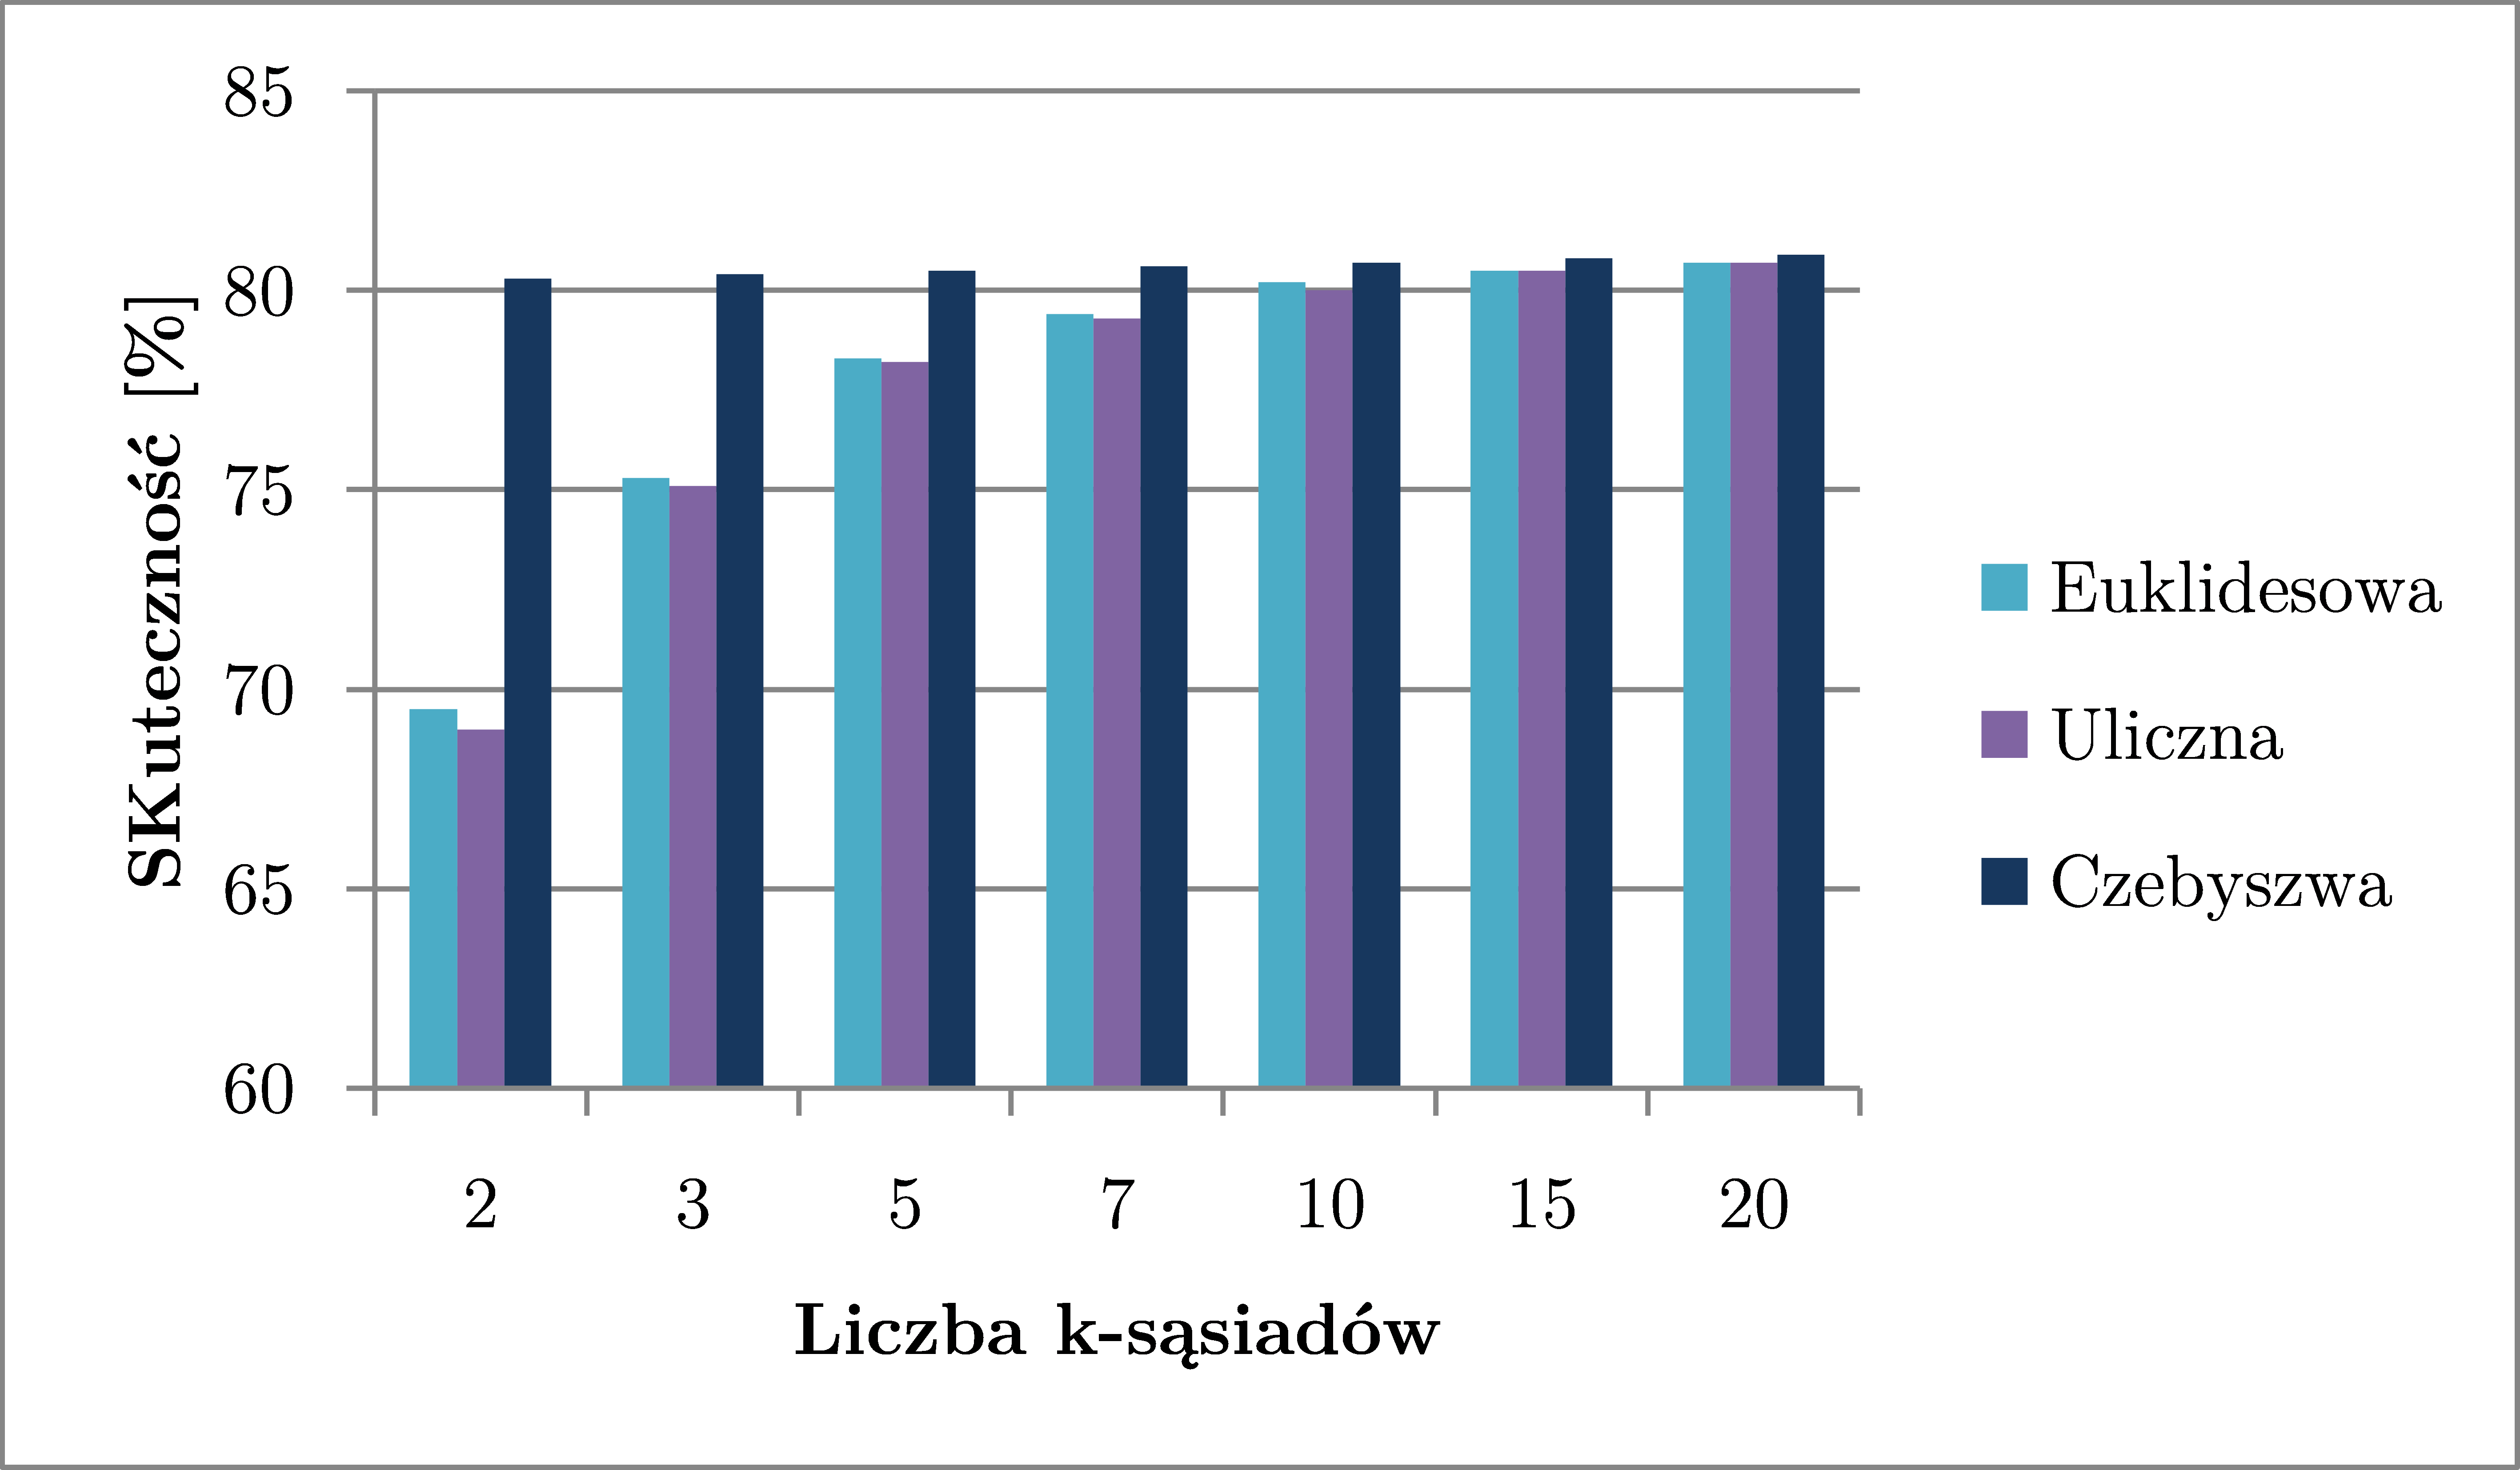
\includegraphics[width=0.9\textwidth]{{Rysunki/OWN-places.png}}
	\caption{Dane z Tabel 7-9 dla kategorii places}
\end{figure}

\begin{figure}[H]
	\centering
	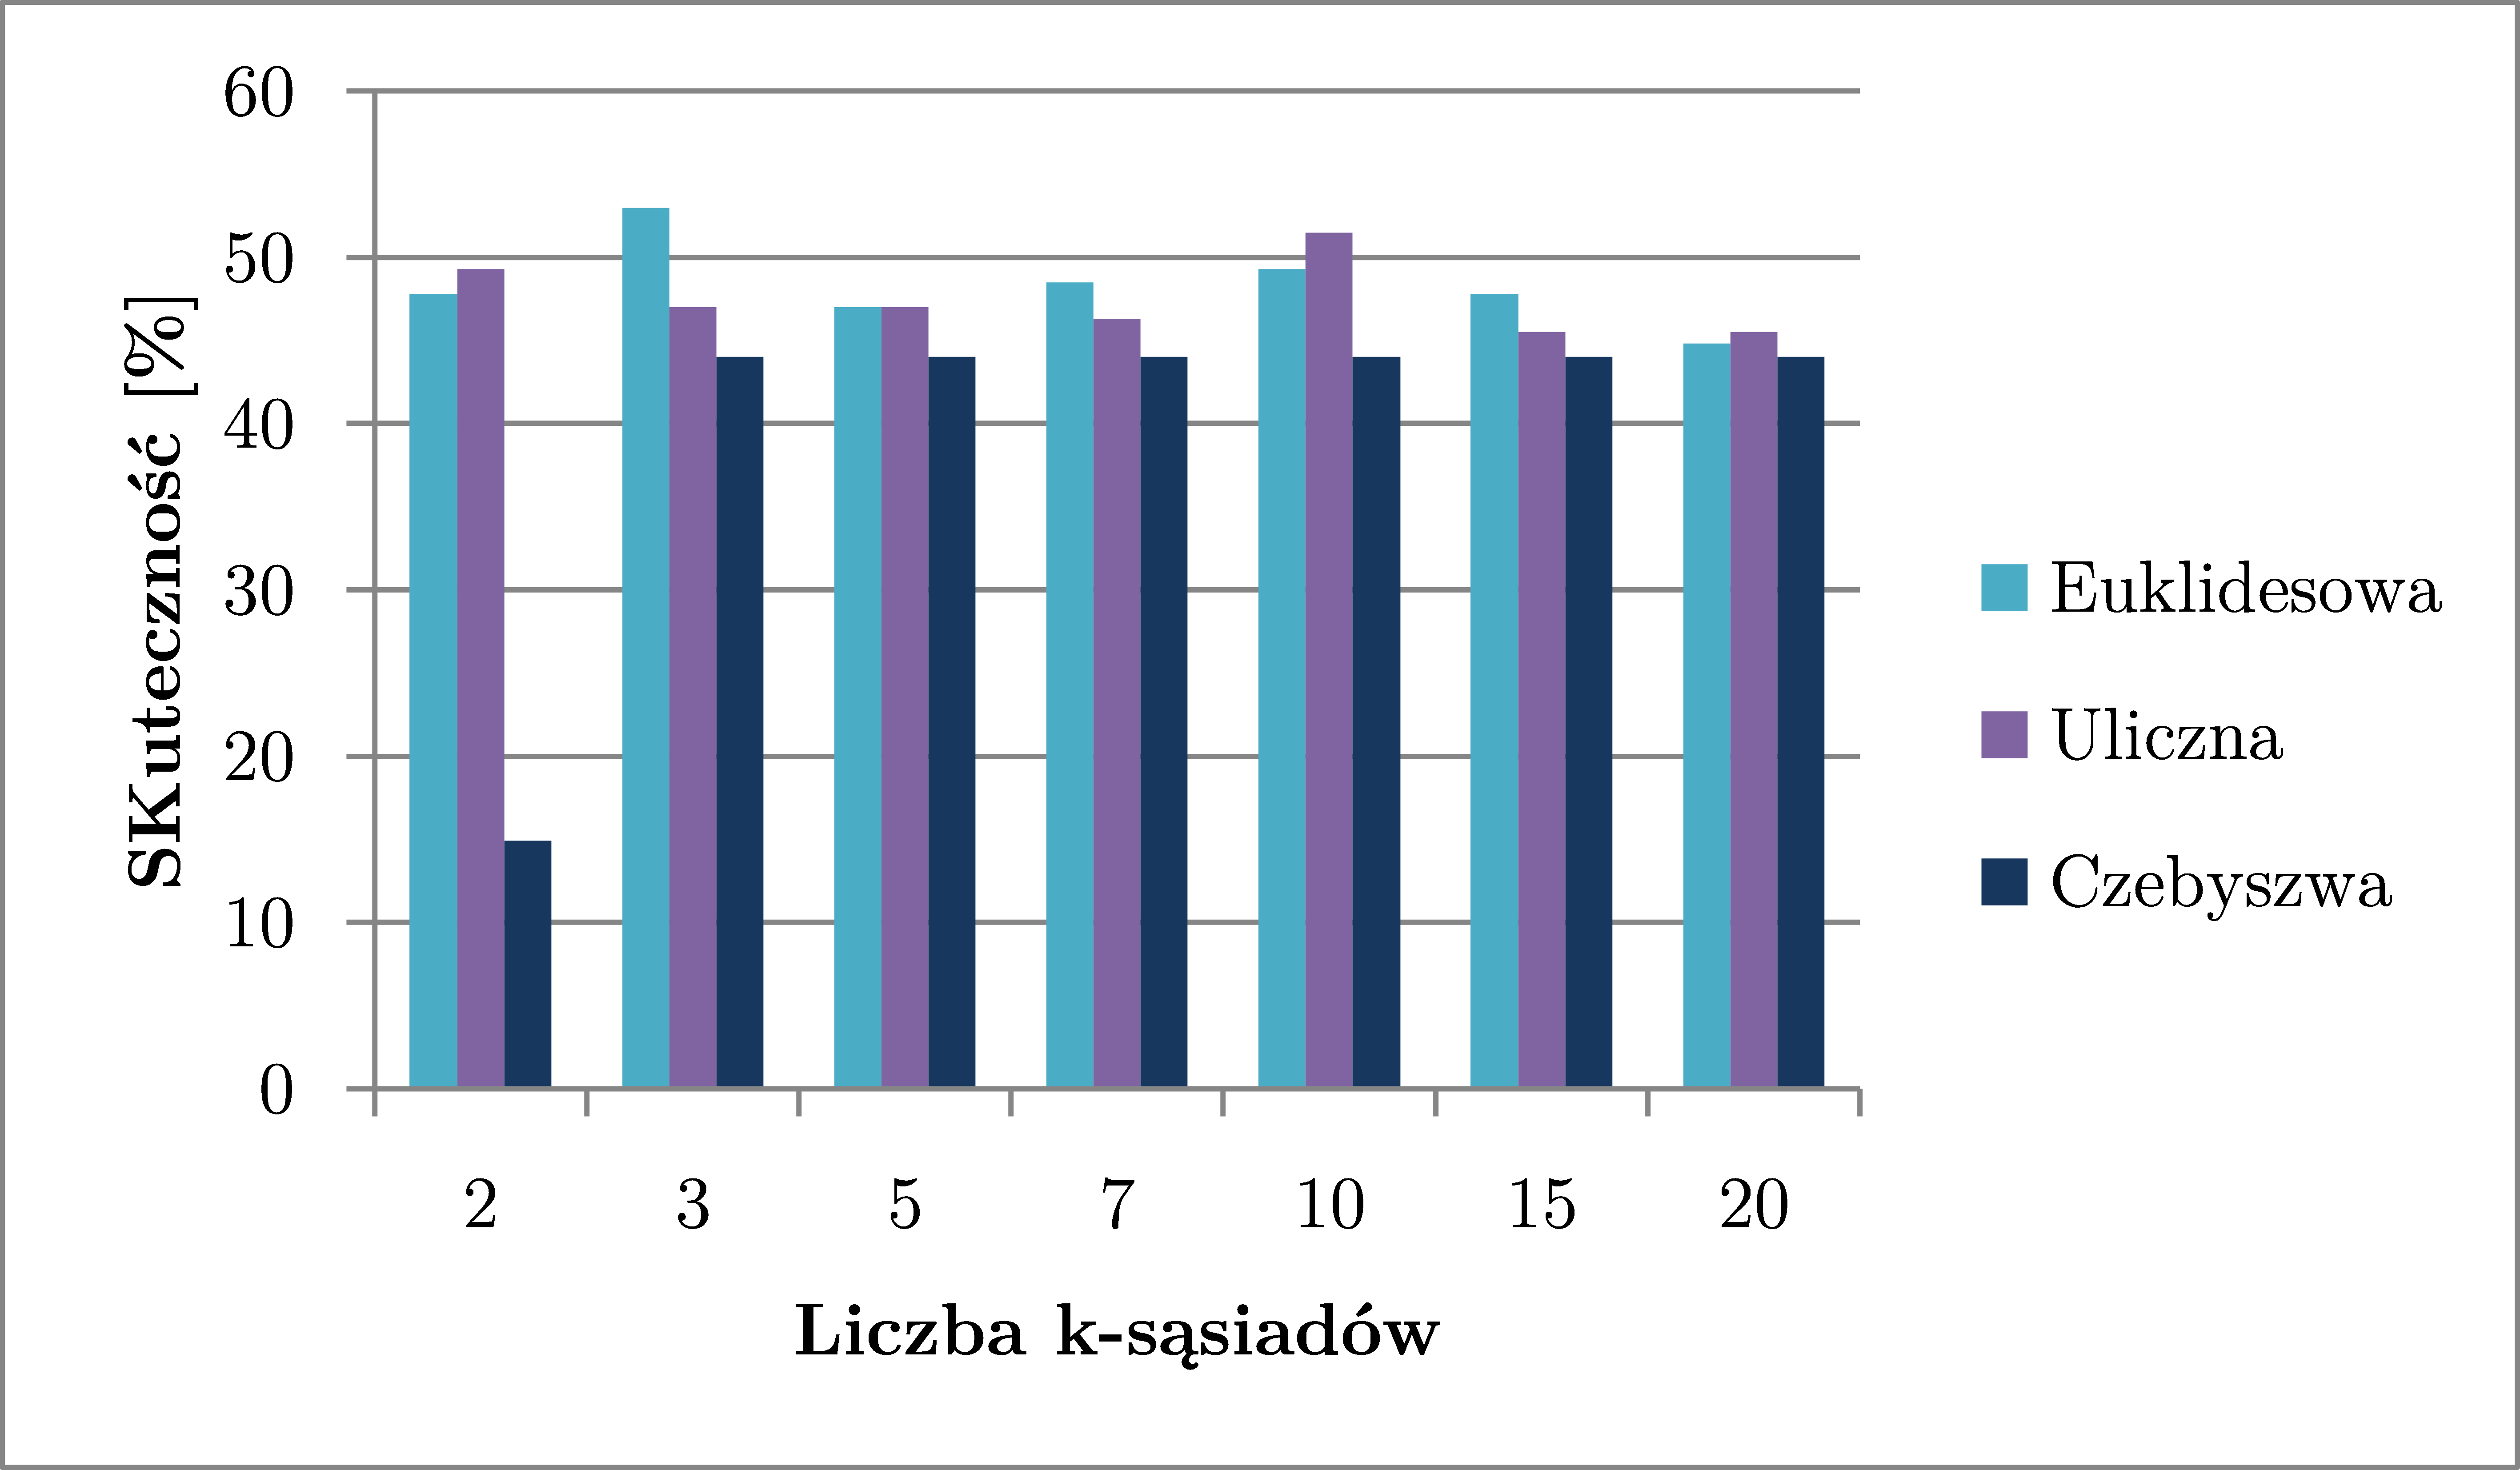
\includegraphics[width=0.9\textwidth]{{Rysunki/OWN-topics.png}}
	\caption{Dane z Tabel 7-9 dla kategorii topics}
\end{figure}

\begin{figure}[H]
	\centering
	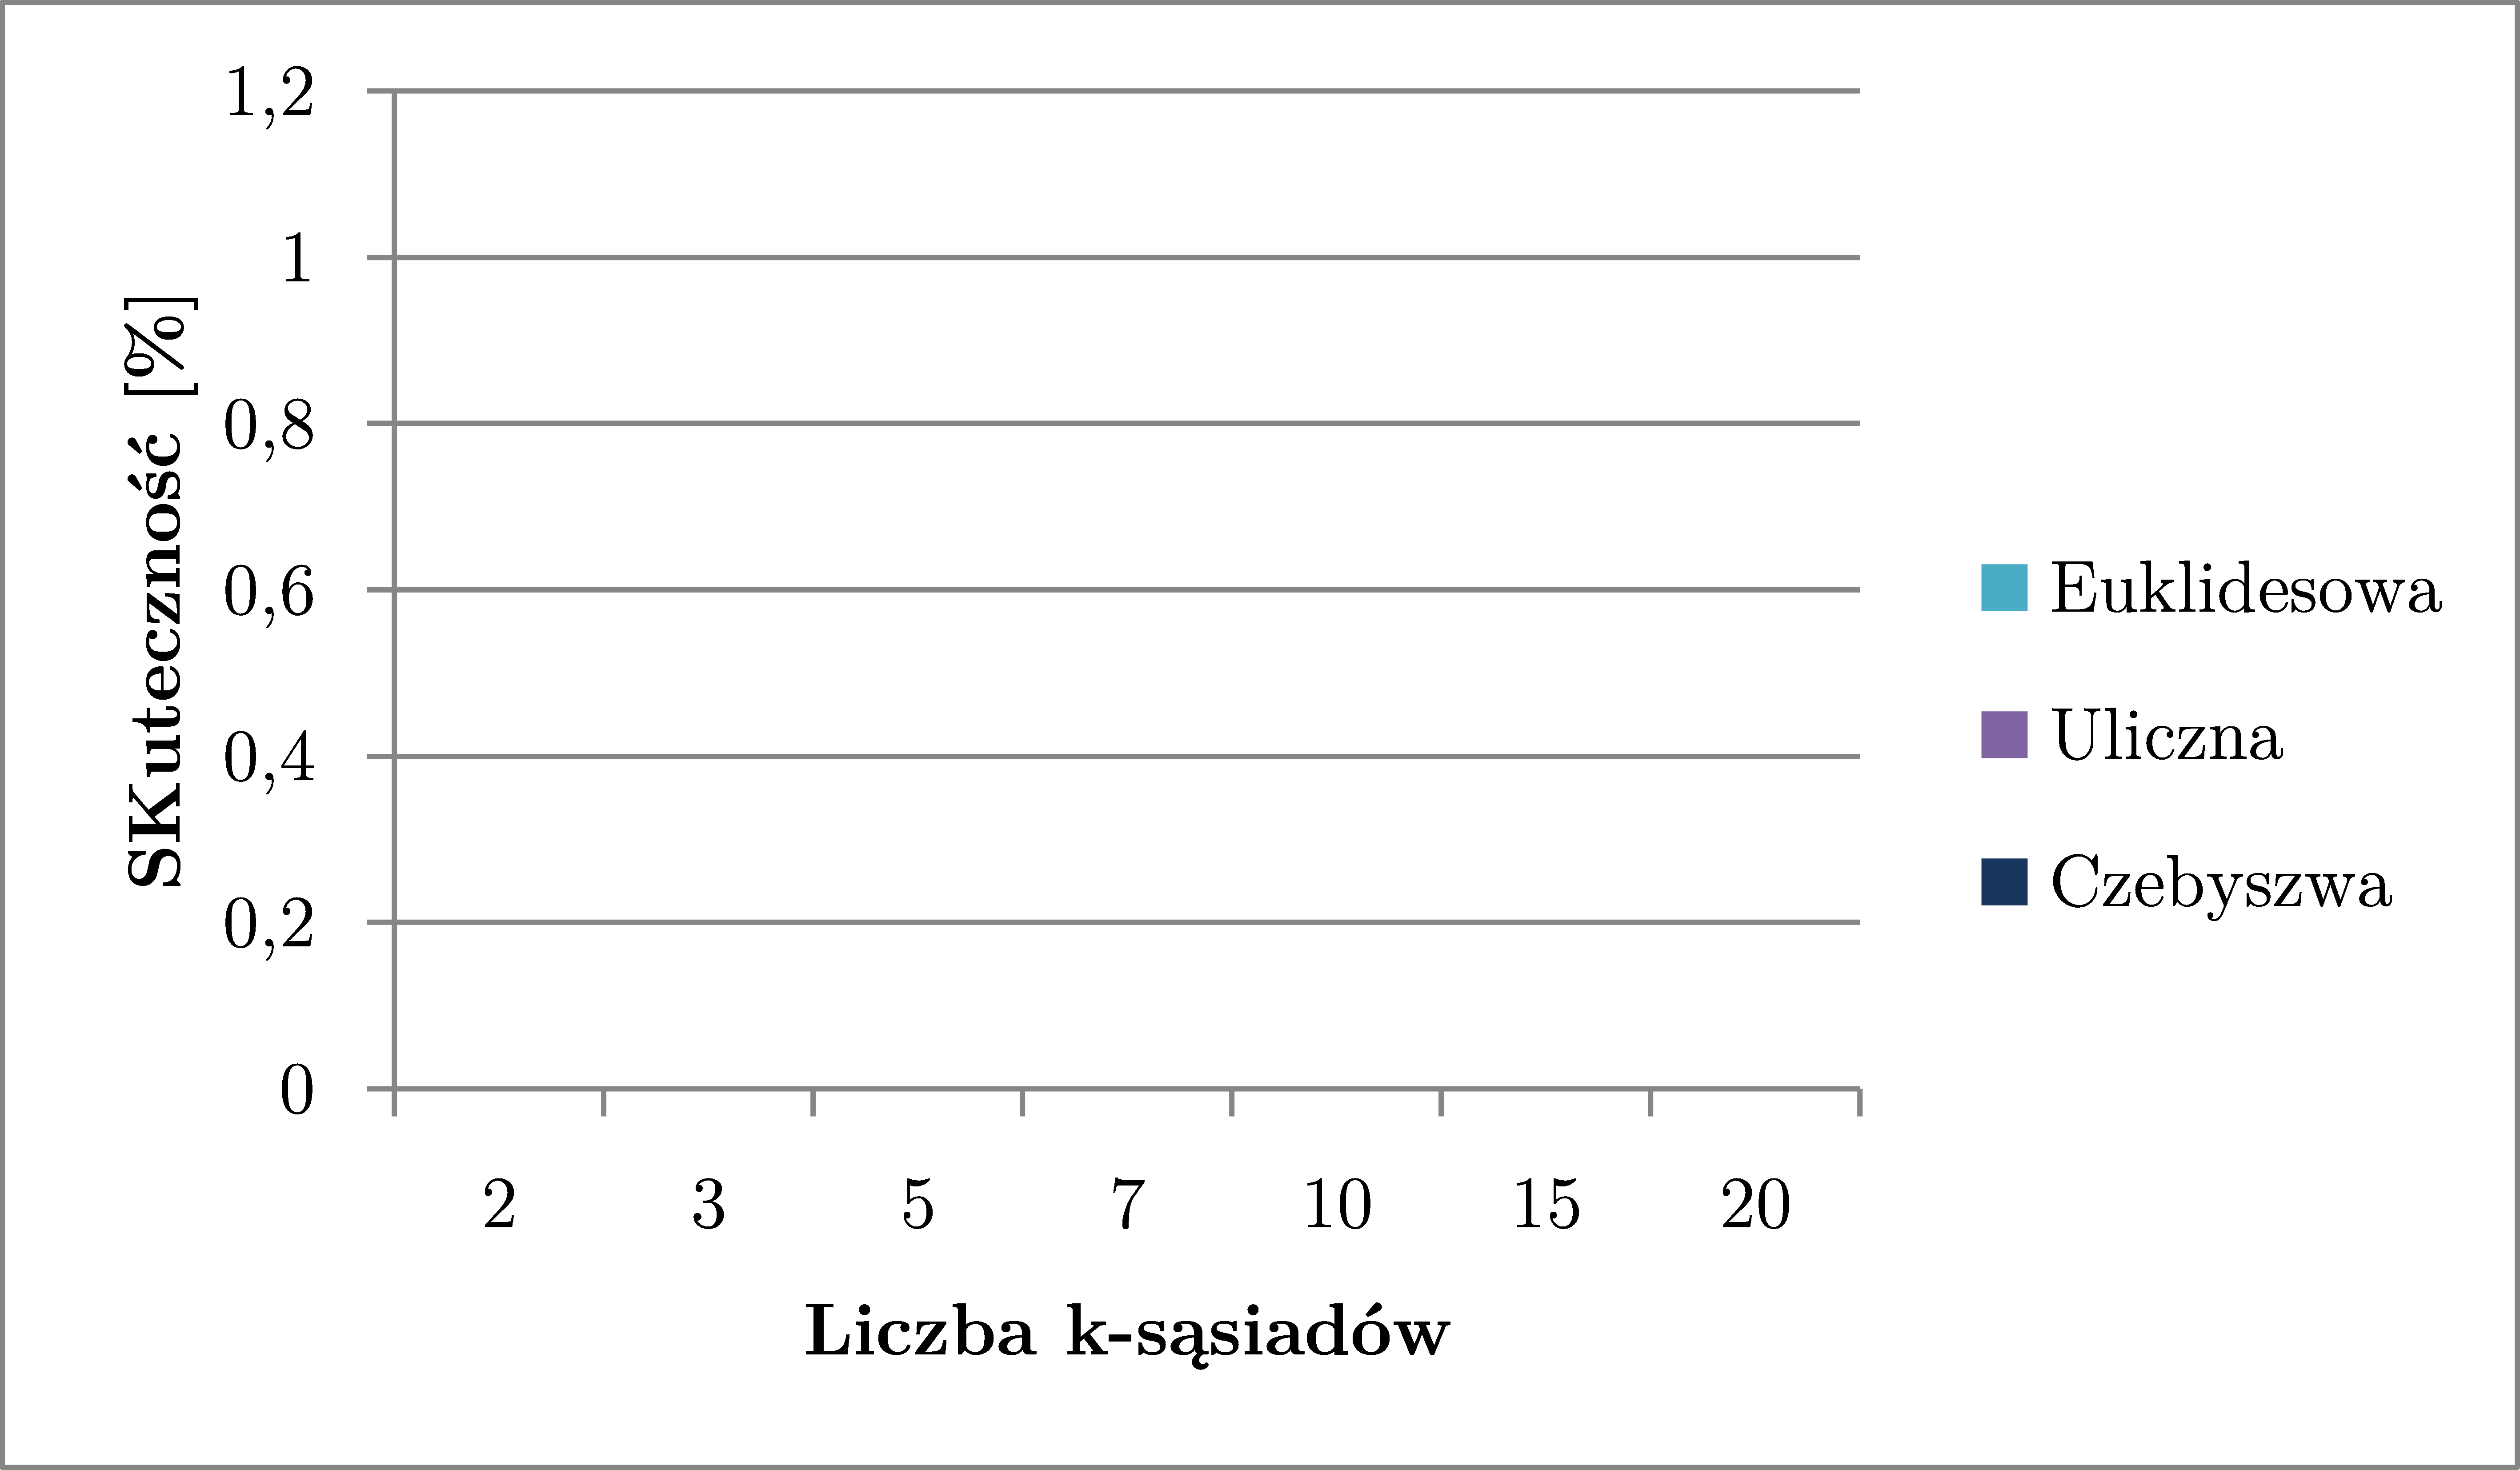
\includegraphics[width=0.9\textwidth]{{Rysunki/OWN-authors.png}}
	\caption{Dane z Tabel 7-9 dla kategorii authors (własne teksty)}
\end{figure}

\subsection{Wpływ podziału tekstów na zbiory treningowe i testowe na klasyfikację}

\begin{table}[H]
	\centering
	\begin{tabular}{c c c c} 
		\hline
		\textbf{k} & \textbf{80\%} & \textbf{60\%} &  \textbf{40\%} \\ [0.5ex] 
		\hline
		\hline 
		5 & 82.7 & 80.2 & 78.4 \\
		7 & 83.3 & 81.0 & 79.9 \\
		10 & 84.2 & 81.5 & 80.4 \\
		15 & 83.9 & 81.6 & 80.4 \\
		\hline
	\end{tabular}
	\caption{Skuteczność klasyfikacji dla pierwszego sposobu ekstrakcji, dla kategorii places}
\end{table}

\begin{figure}[H]
	\centering
	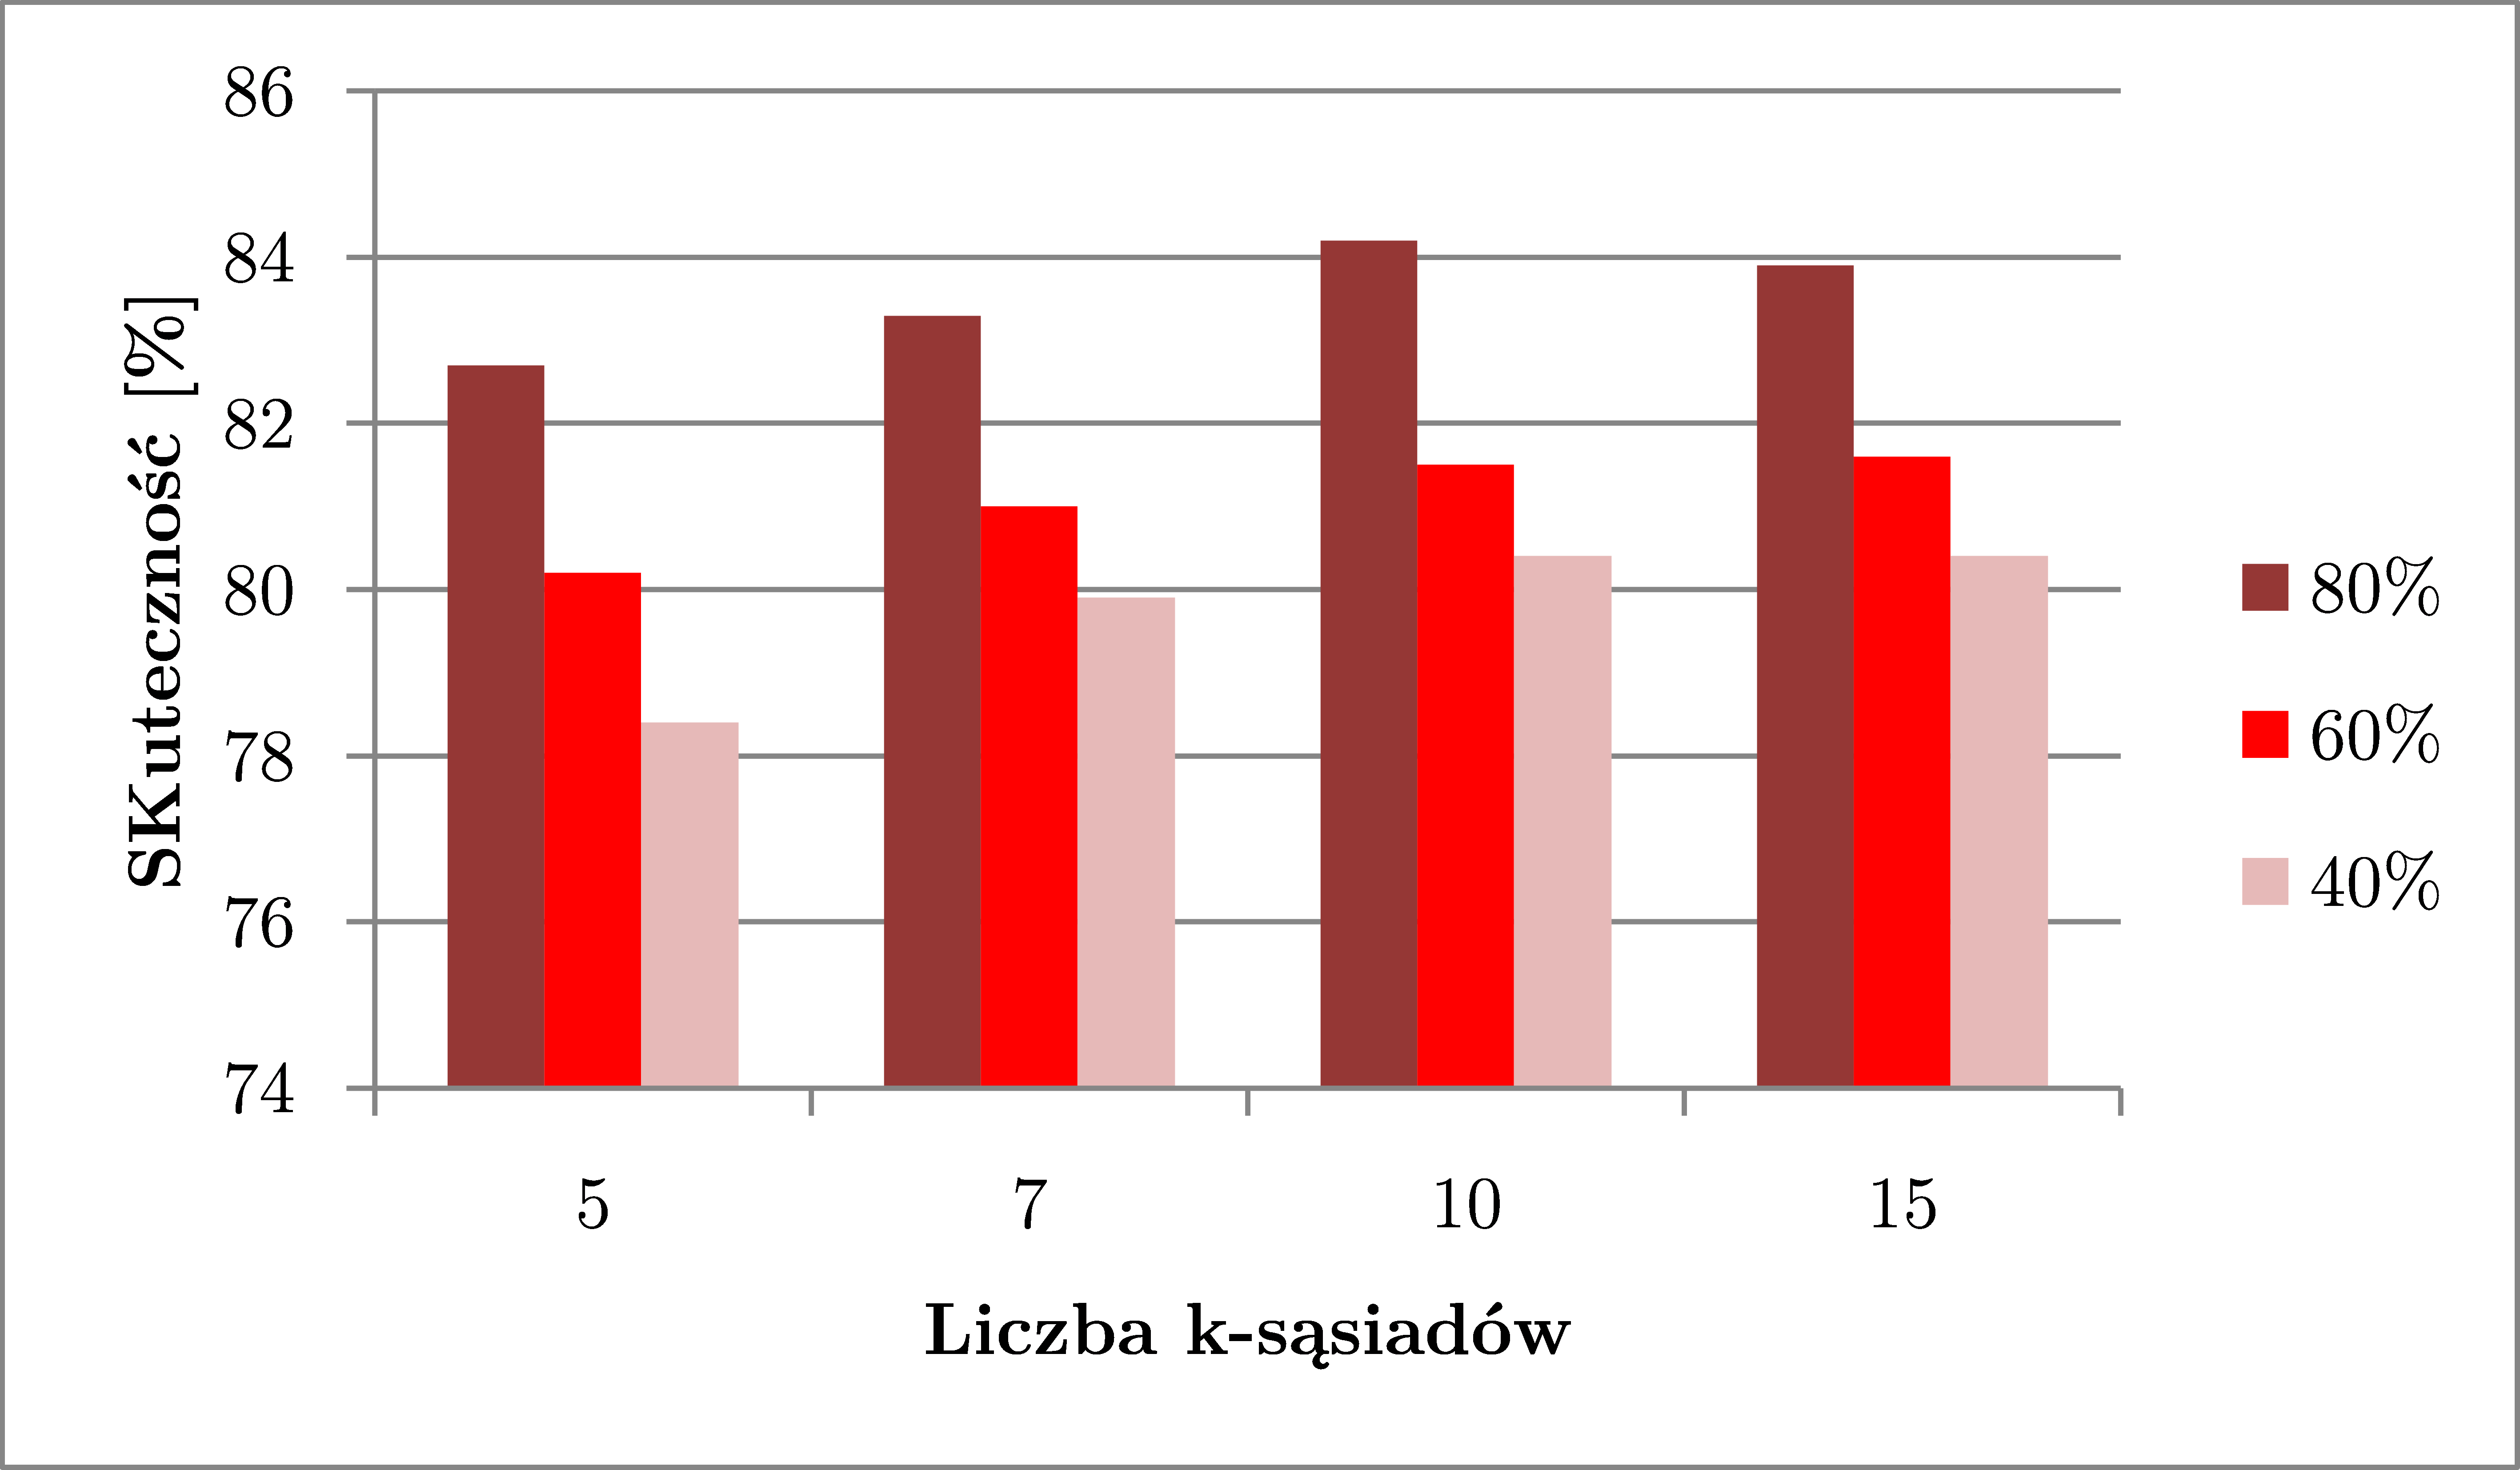
\includegraphics[width=0.9\textwidth]{{Rysunki/TF-80-60-40-places.png}}
	\caption{Skuteczność klasyfikacji dla pierwszego sposobu ekstrakcji, dla kategorii places}
\end{figure}

\begin{table}[H]
	\centering
	\begin{tabular}{c c c c} 
		\hline
		\textbf{k} & \textbf{80\%} & \textbf{60\%} &  \textbf{40\%} \\ [0.5ex] 
		\hline
		\hline 
		7 & 56.7 & 53.7 & 62.7 \\
		10 & 59.7 & 60.4 & 62.2 \\
		15 & 58.2 & 62.7 & 64.7 \\
		20 & 62.7 & 61.2 & 64.7 \\
		\hline
	\end{tabular}
	\caption{Skuteczność klasyfikacji dla pierwszego sposobu ekstrakcji, dla kategorii topics}
\end{table}

\begin{figure}[H]
	\centering
	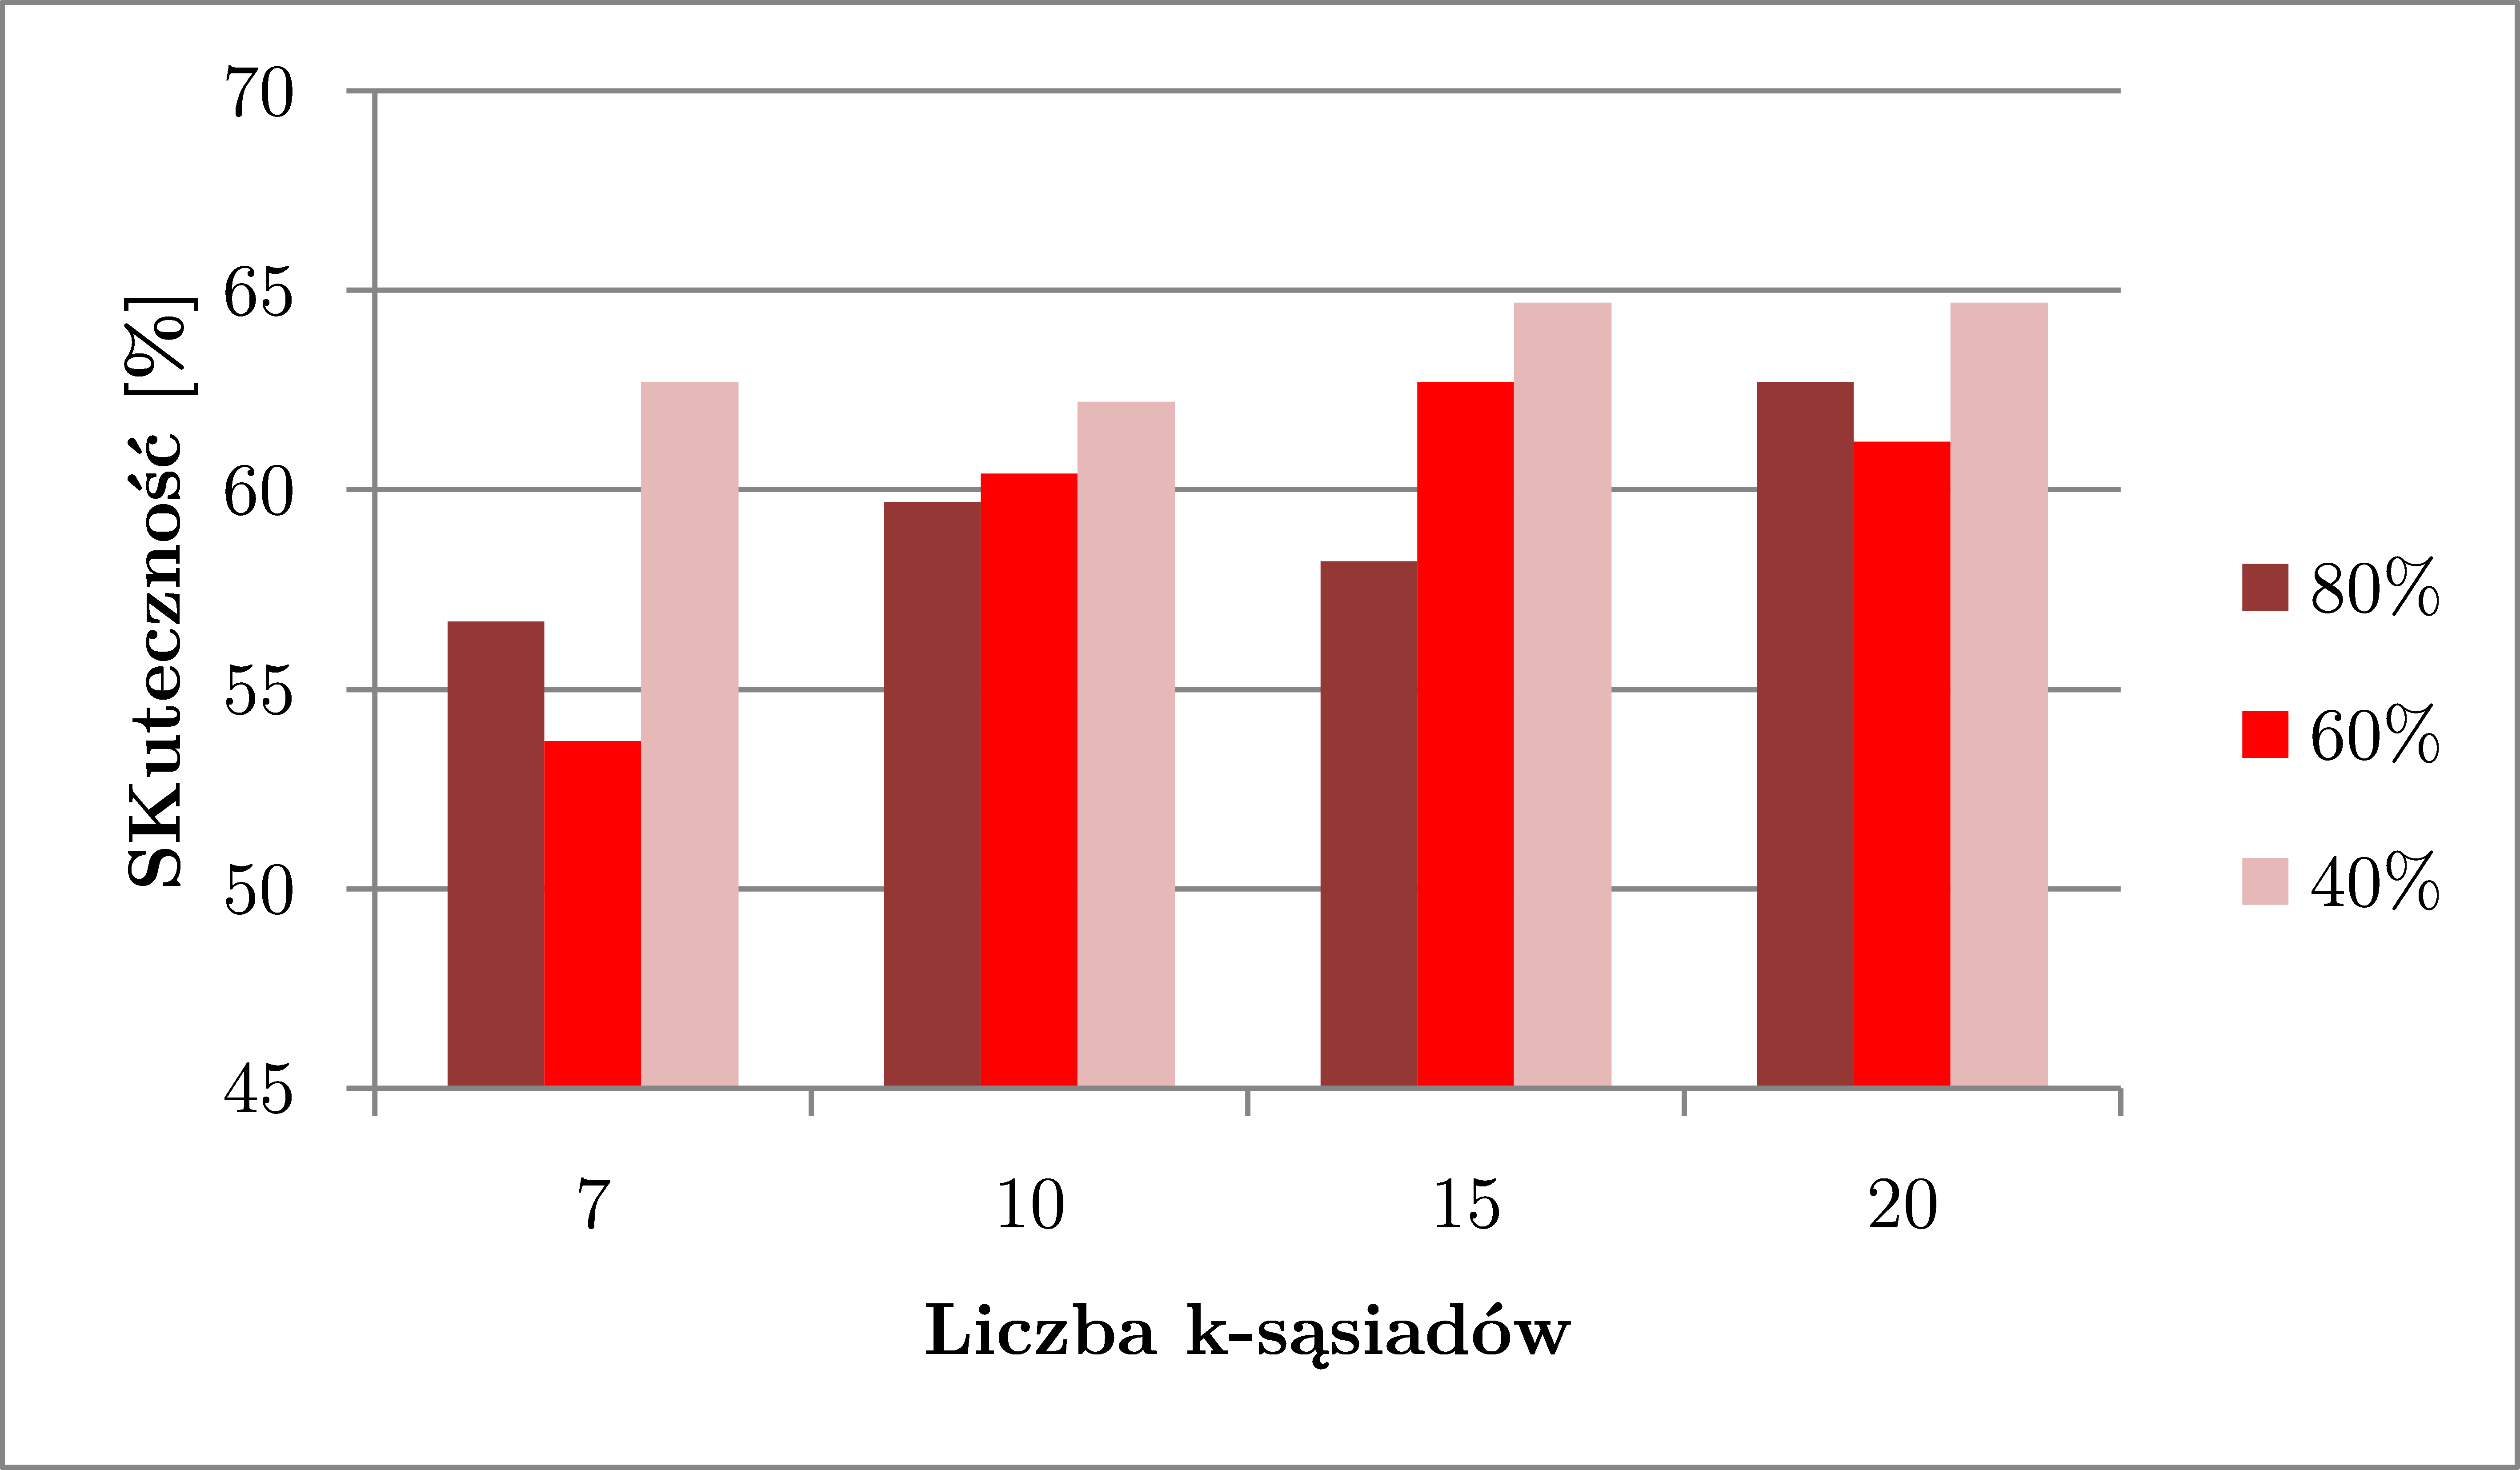
\includegraphics[width=0.9\textwidth]{{Rysunki/TF-80-60-40-topics.png}}
	\caption{Skuteczność klasyfikacji dla pierwszego sposobu ekstrakcji, dla kategorii topics}
\end{figure}

\begin{table}[H]
	\centering
	\begin{tabular}{c c c c} 
		\hline
		\textbf{k} & \textbf{80\%} & \textbf{60\%} &  \textbf{40\%} \\ [0.5ex] 
		\hline
		\hline 
		2 & 19.0 & 43.9 & 38.7 \\
		3 & 19.0 & 43.9 & 37.1 \\
		5 & 23.8 & 36.6 & 29.0 \\
		7 & 14.3 & 26.8 & 32.3 \\
		\hline
	\end{tabular}
	\caption{Skuteczność klasyfikacji dla pierwszego sposobu ekstrakcji, dla kategorii authors}
\end{table}

\begin{figure}[H]
	\centering
	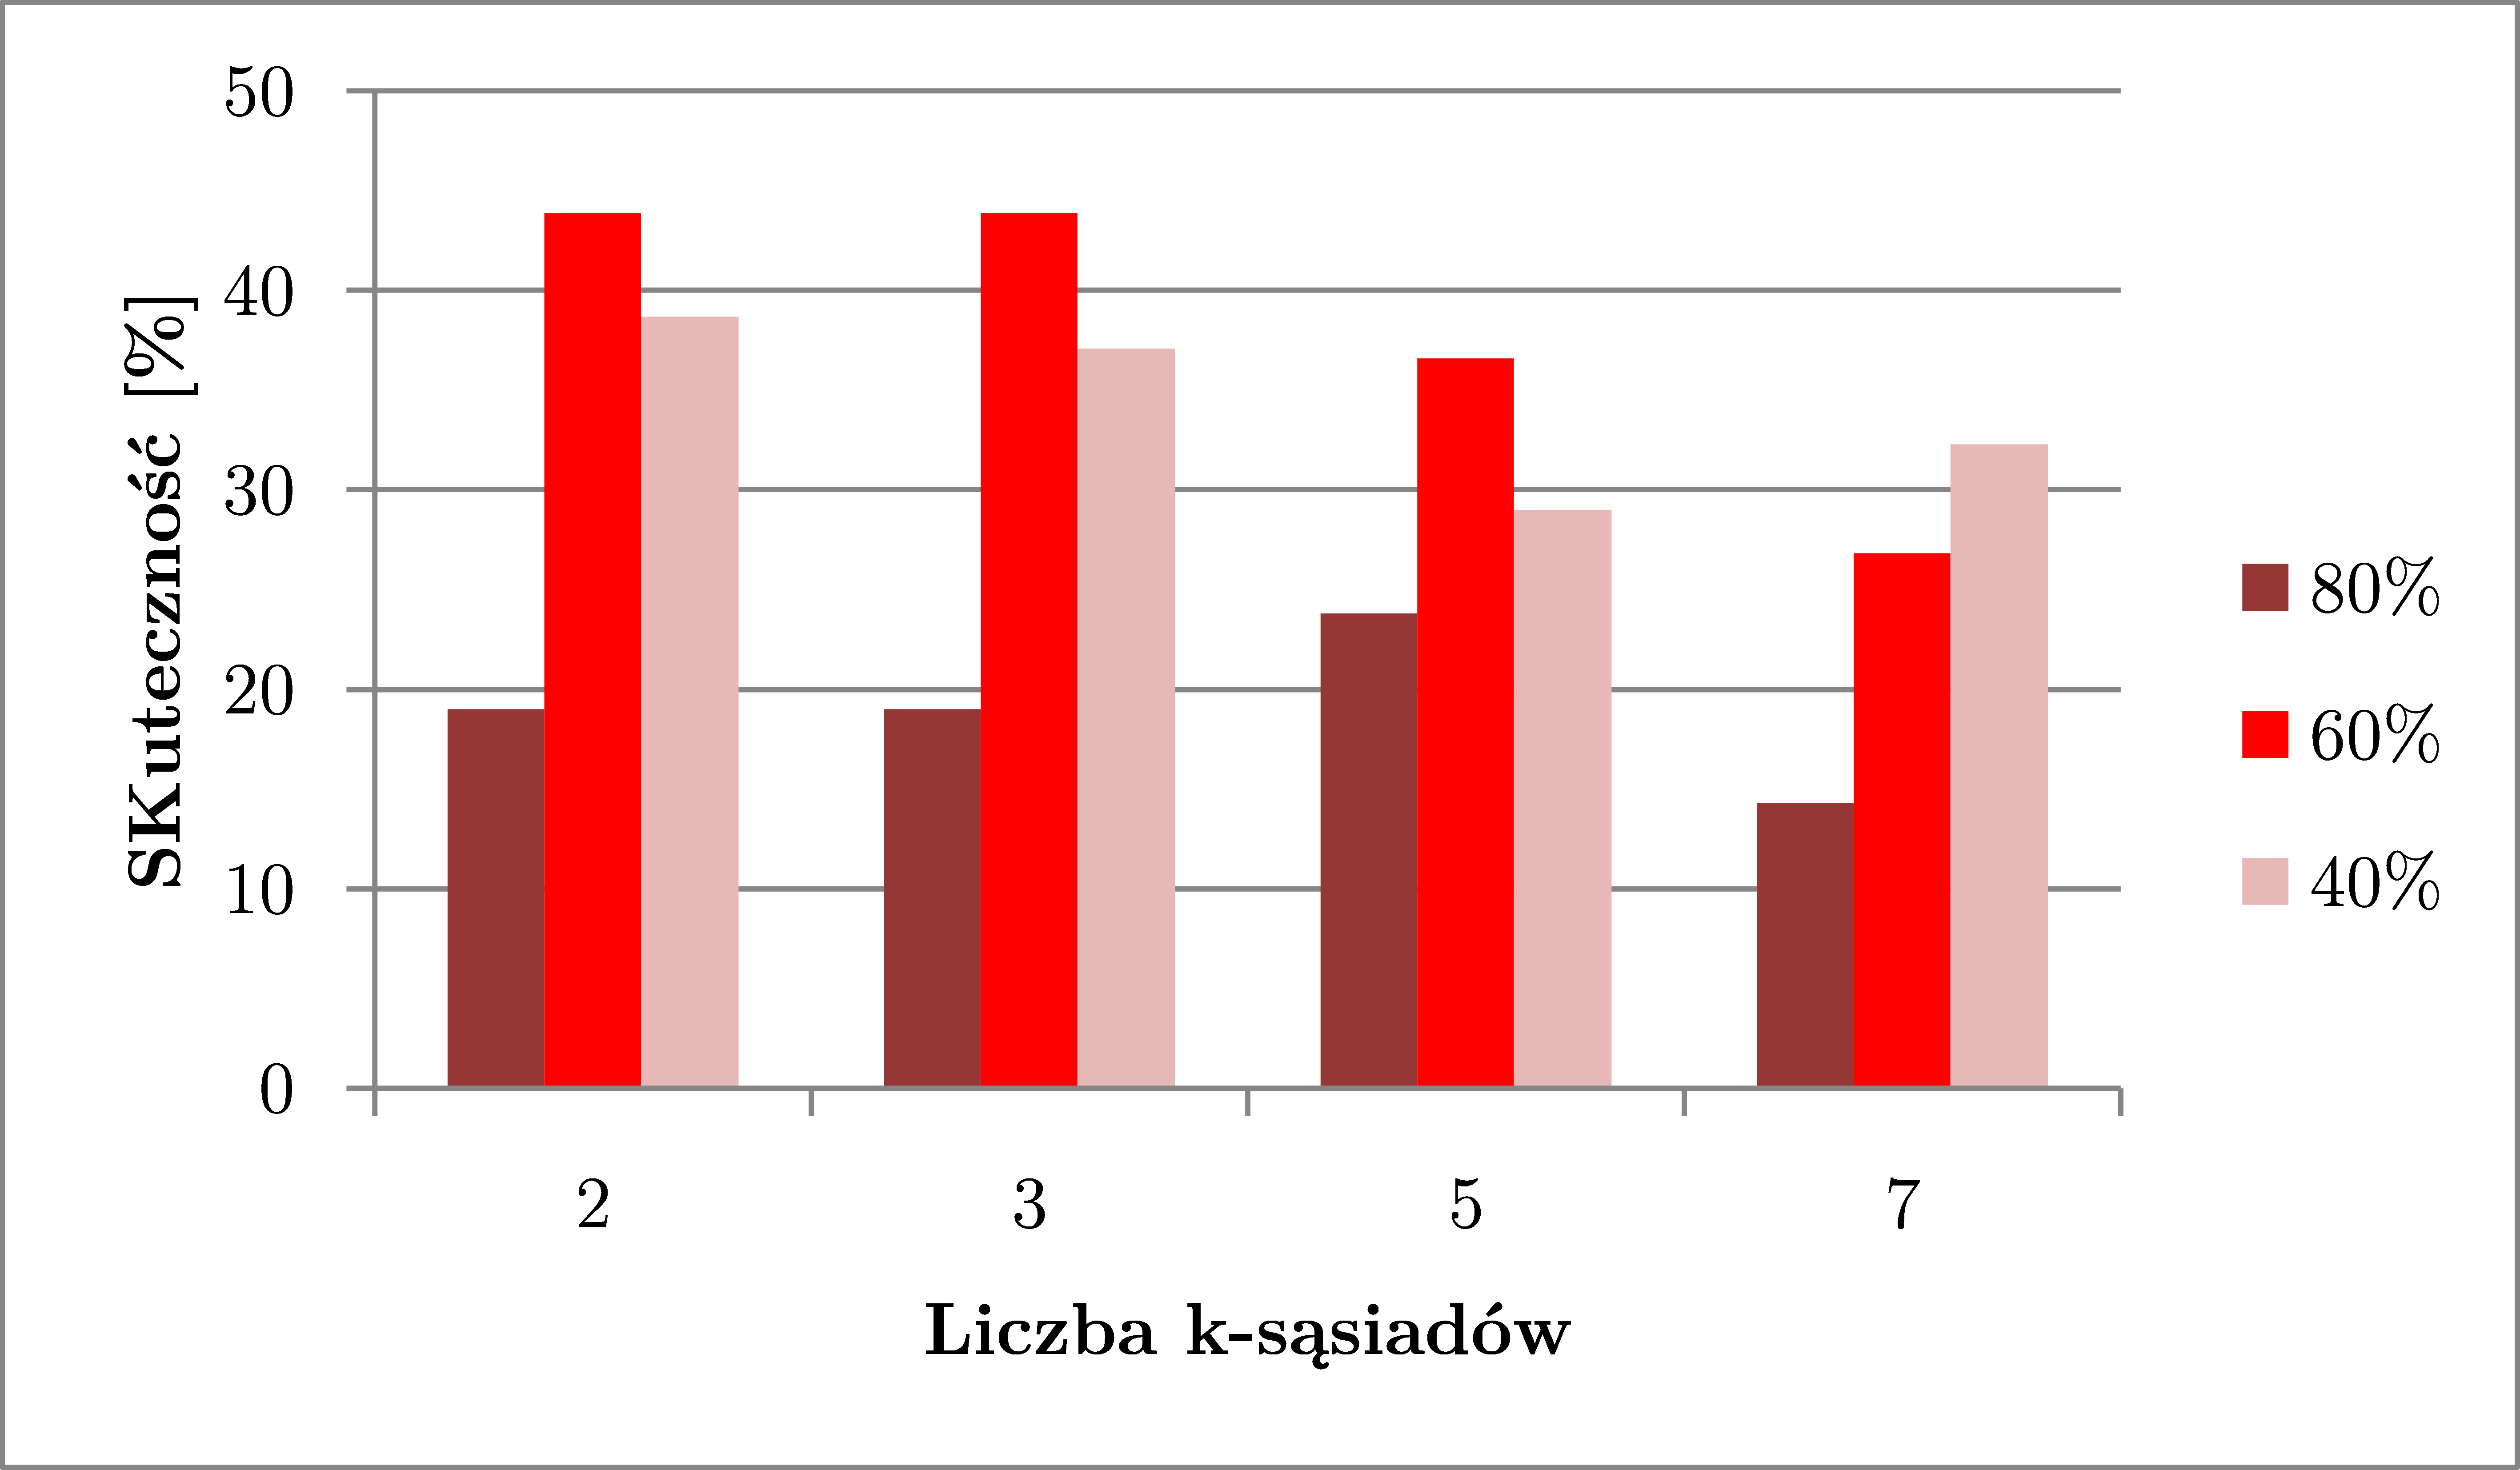
\includegraphics[width=0.9\textwidth]{{Rysunki/TF-80-60-40-authors.png}}
	\caption{Skuteczność klasyfikacji dla pierwszego sposobu ekstrakcji, dla kategorii authors}
\end{figure}


\begin{table}[H]
	\centering
	\begin{tabular}{c c c c} 
		\hline
		\textbf{k} & \textbf{places [\%]} & \textbf{topics [\%]} &  \textbf{authors [\%]} \\ [0.5ex] 
		\hline
		\hline 
		5 &  &  &  \\
		7 &  &  &  \\
		10 &  &  &  \\
		15 &  &  &  \\
		\hline
	\end{tabular}
	\caption{Skuteczność klasyfikacji dla 80\% danych treningowych dla drugiego sposobu ekstrakcji}
\end{table}

\begin{table}[H]
	\centering
	\begin{tabular}{c c c c} 
		\hline
		\textbf{k} & \textbf{places [\%]} & \textbf{topics [\%]} &  \textbf{authors [\%]} \\ [0.5ex] 
		\hline
		\hline 
		5 &  &  &  \\
		7 &  &  &  \\
		10 &  &  &  \\
		15 &  &  &  \\
		\hline
	\end{tabular}
	\caption{Skuteczność klasyfikacji dla 60\% danych treningowych dla drugiego sposobu ekstrakcji}
\end{table}

\begin{table}[H]
	\centering
	\begin{tabular}{c c c c} 
		\hline
		\textbf{k} & \textbf{places [\%]} & \textbf{topics [\%]} &  \textbf{authors [\%]} \\ [0.5ex] 
		\hline
		\hline 
		5 &  &  &  \\
		7 &  &  &  \\
		10 &  &  &  \\
		15 &  &  &  \\
		\hline
	\end{tabular}
	\caption{Skuteczność klasyfikacji dla 40\% danych treningowych dla drugiego sposobu ekstrakcji}
\end{table}

\begin{figure}[H]
	\centering
	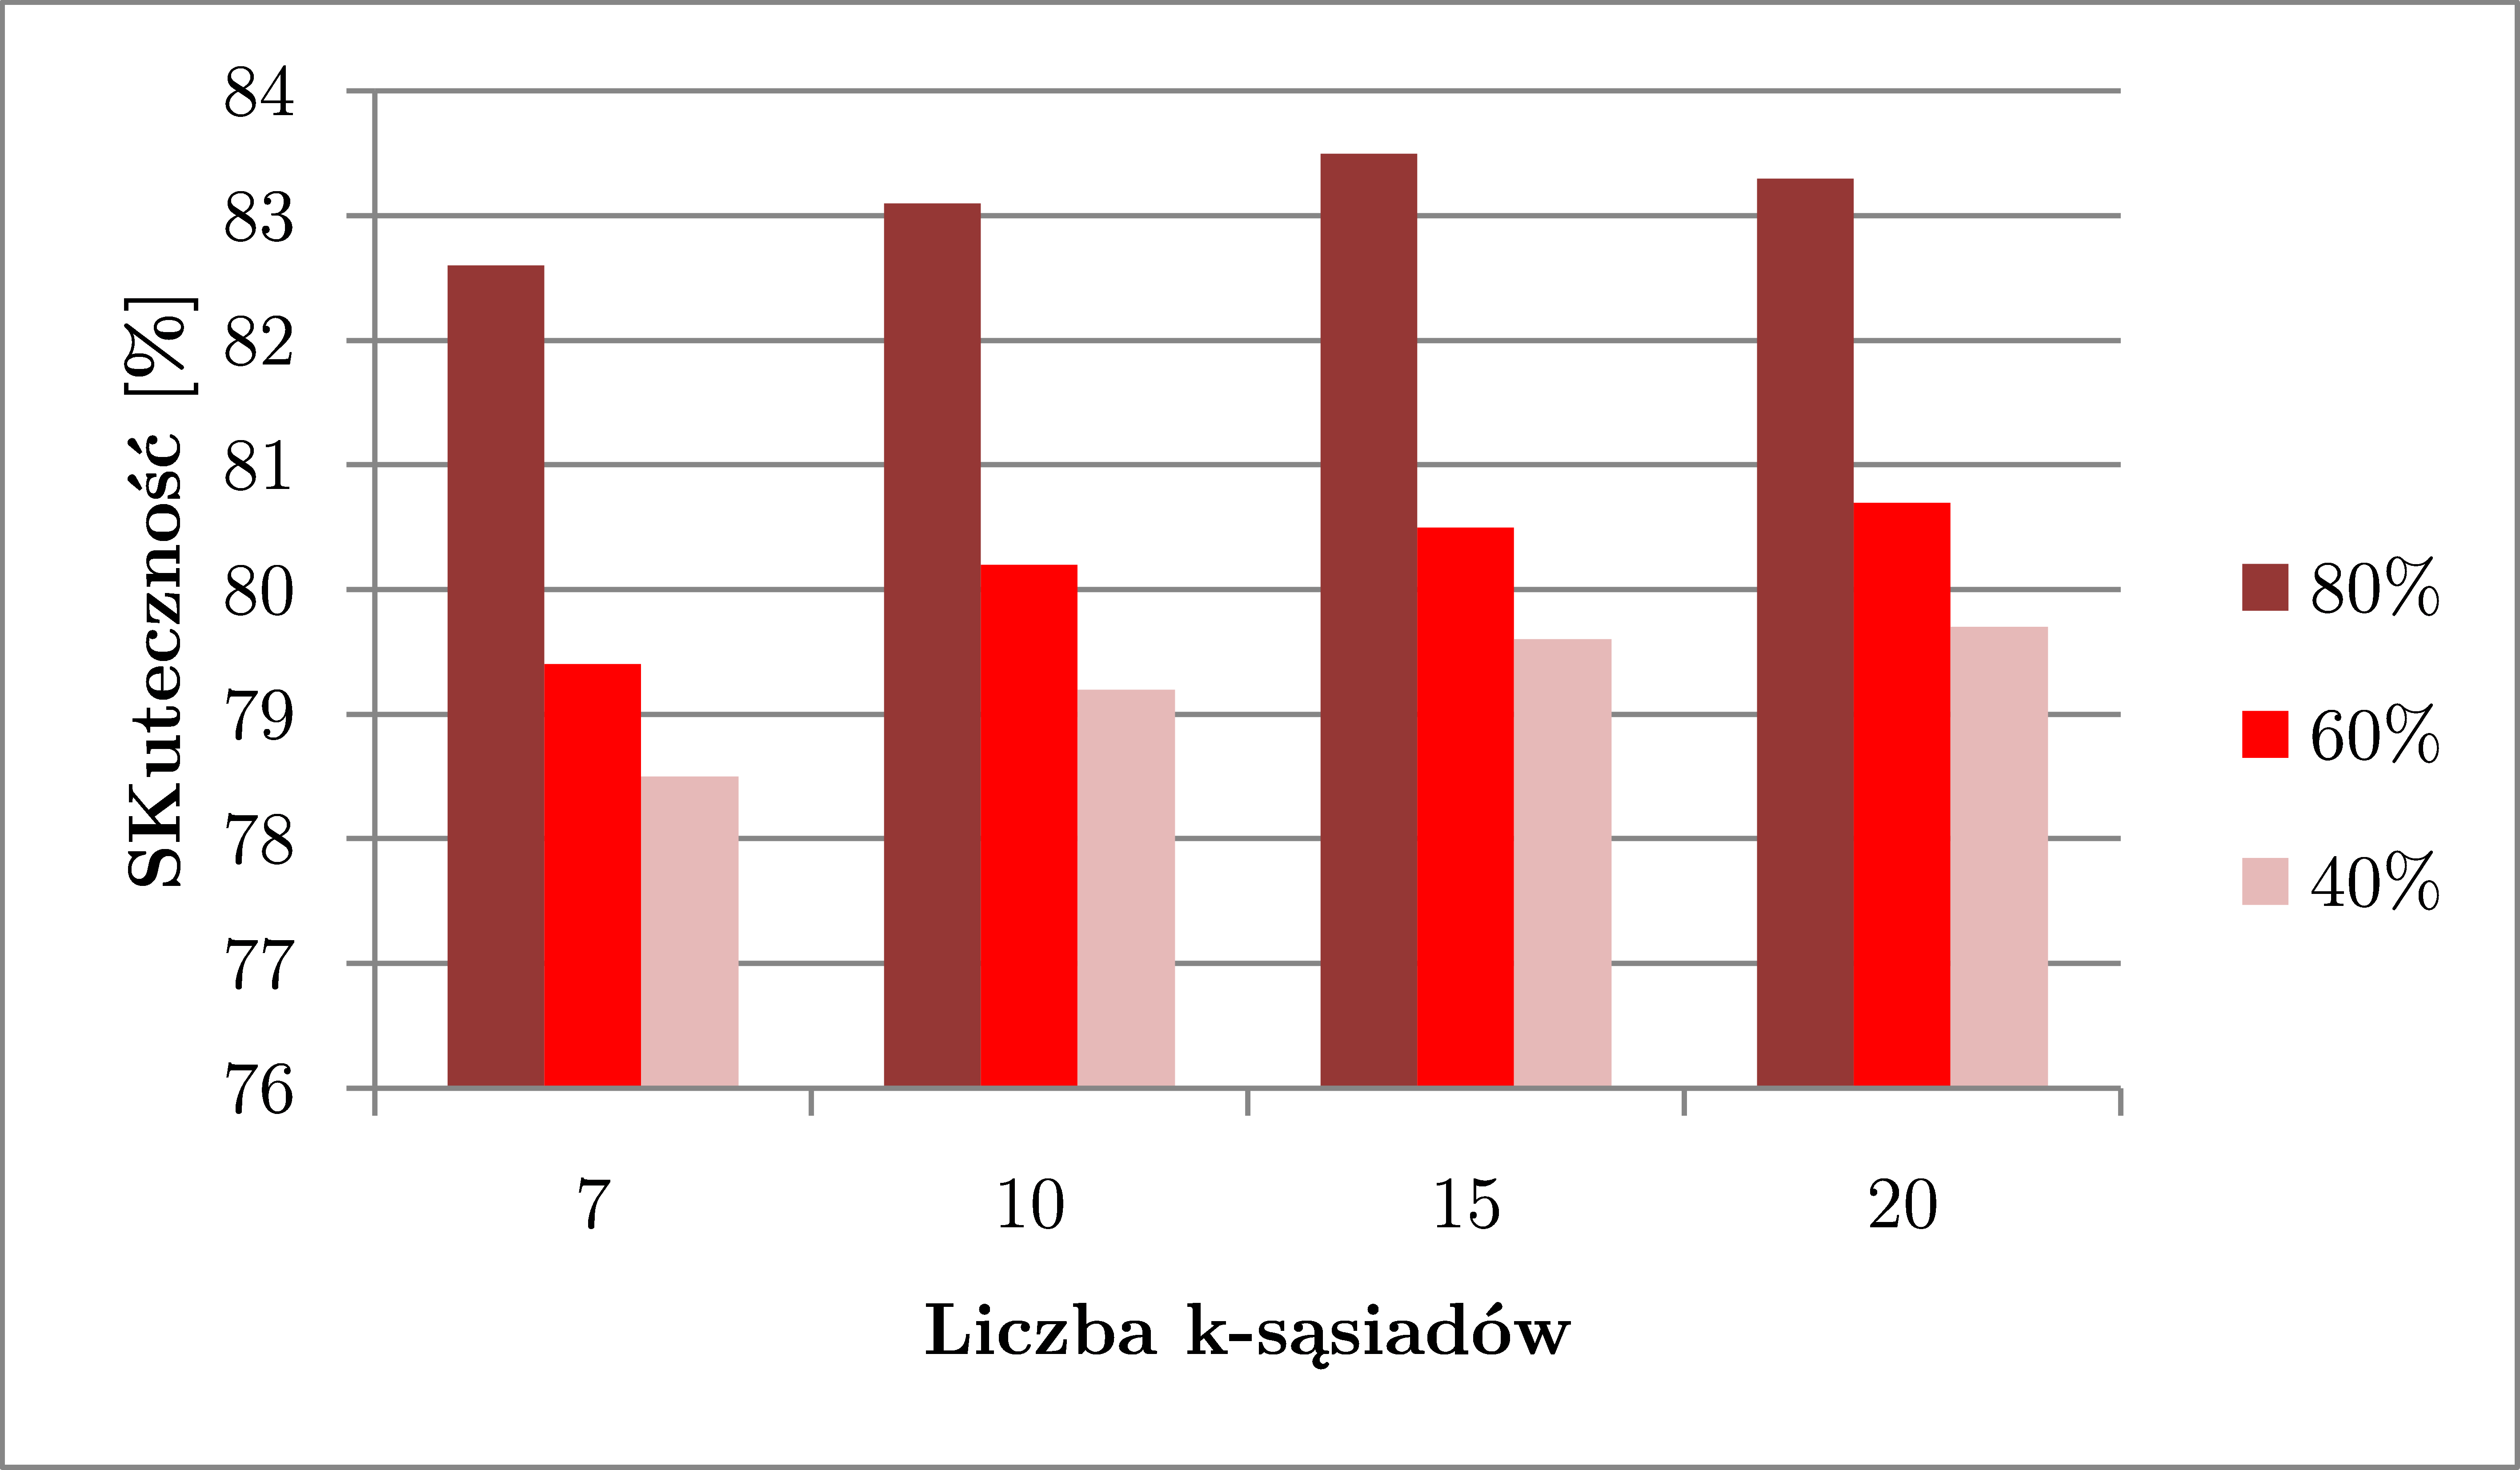
\includegraphics[width=0.9\textwidth]{{Rysunki/OWN-80-60-40-places.png}}
	\caption{Dane z Tabel 13-15 dla kategorii places}
\end{figure}

\begin{figure}[H]
	\centering
	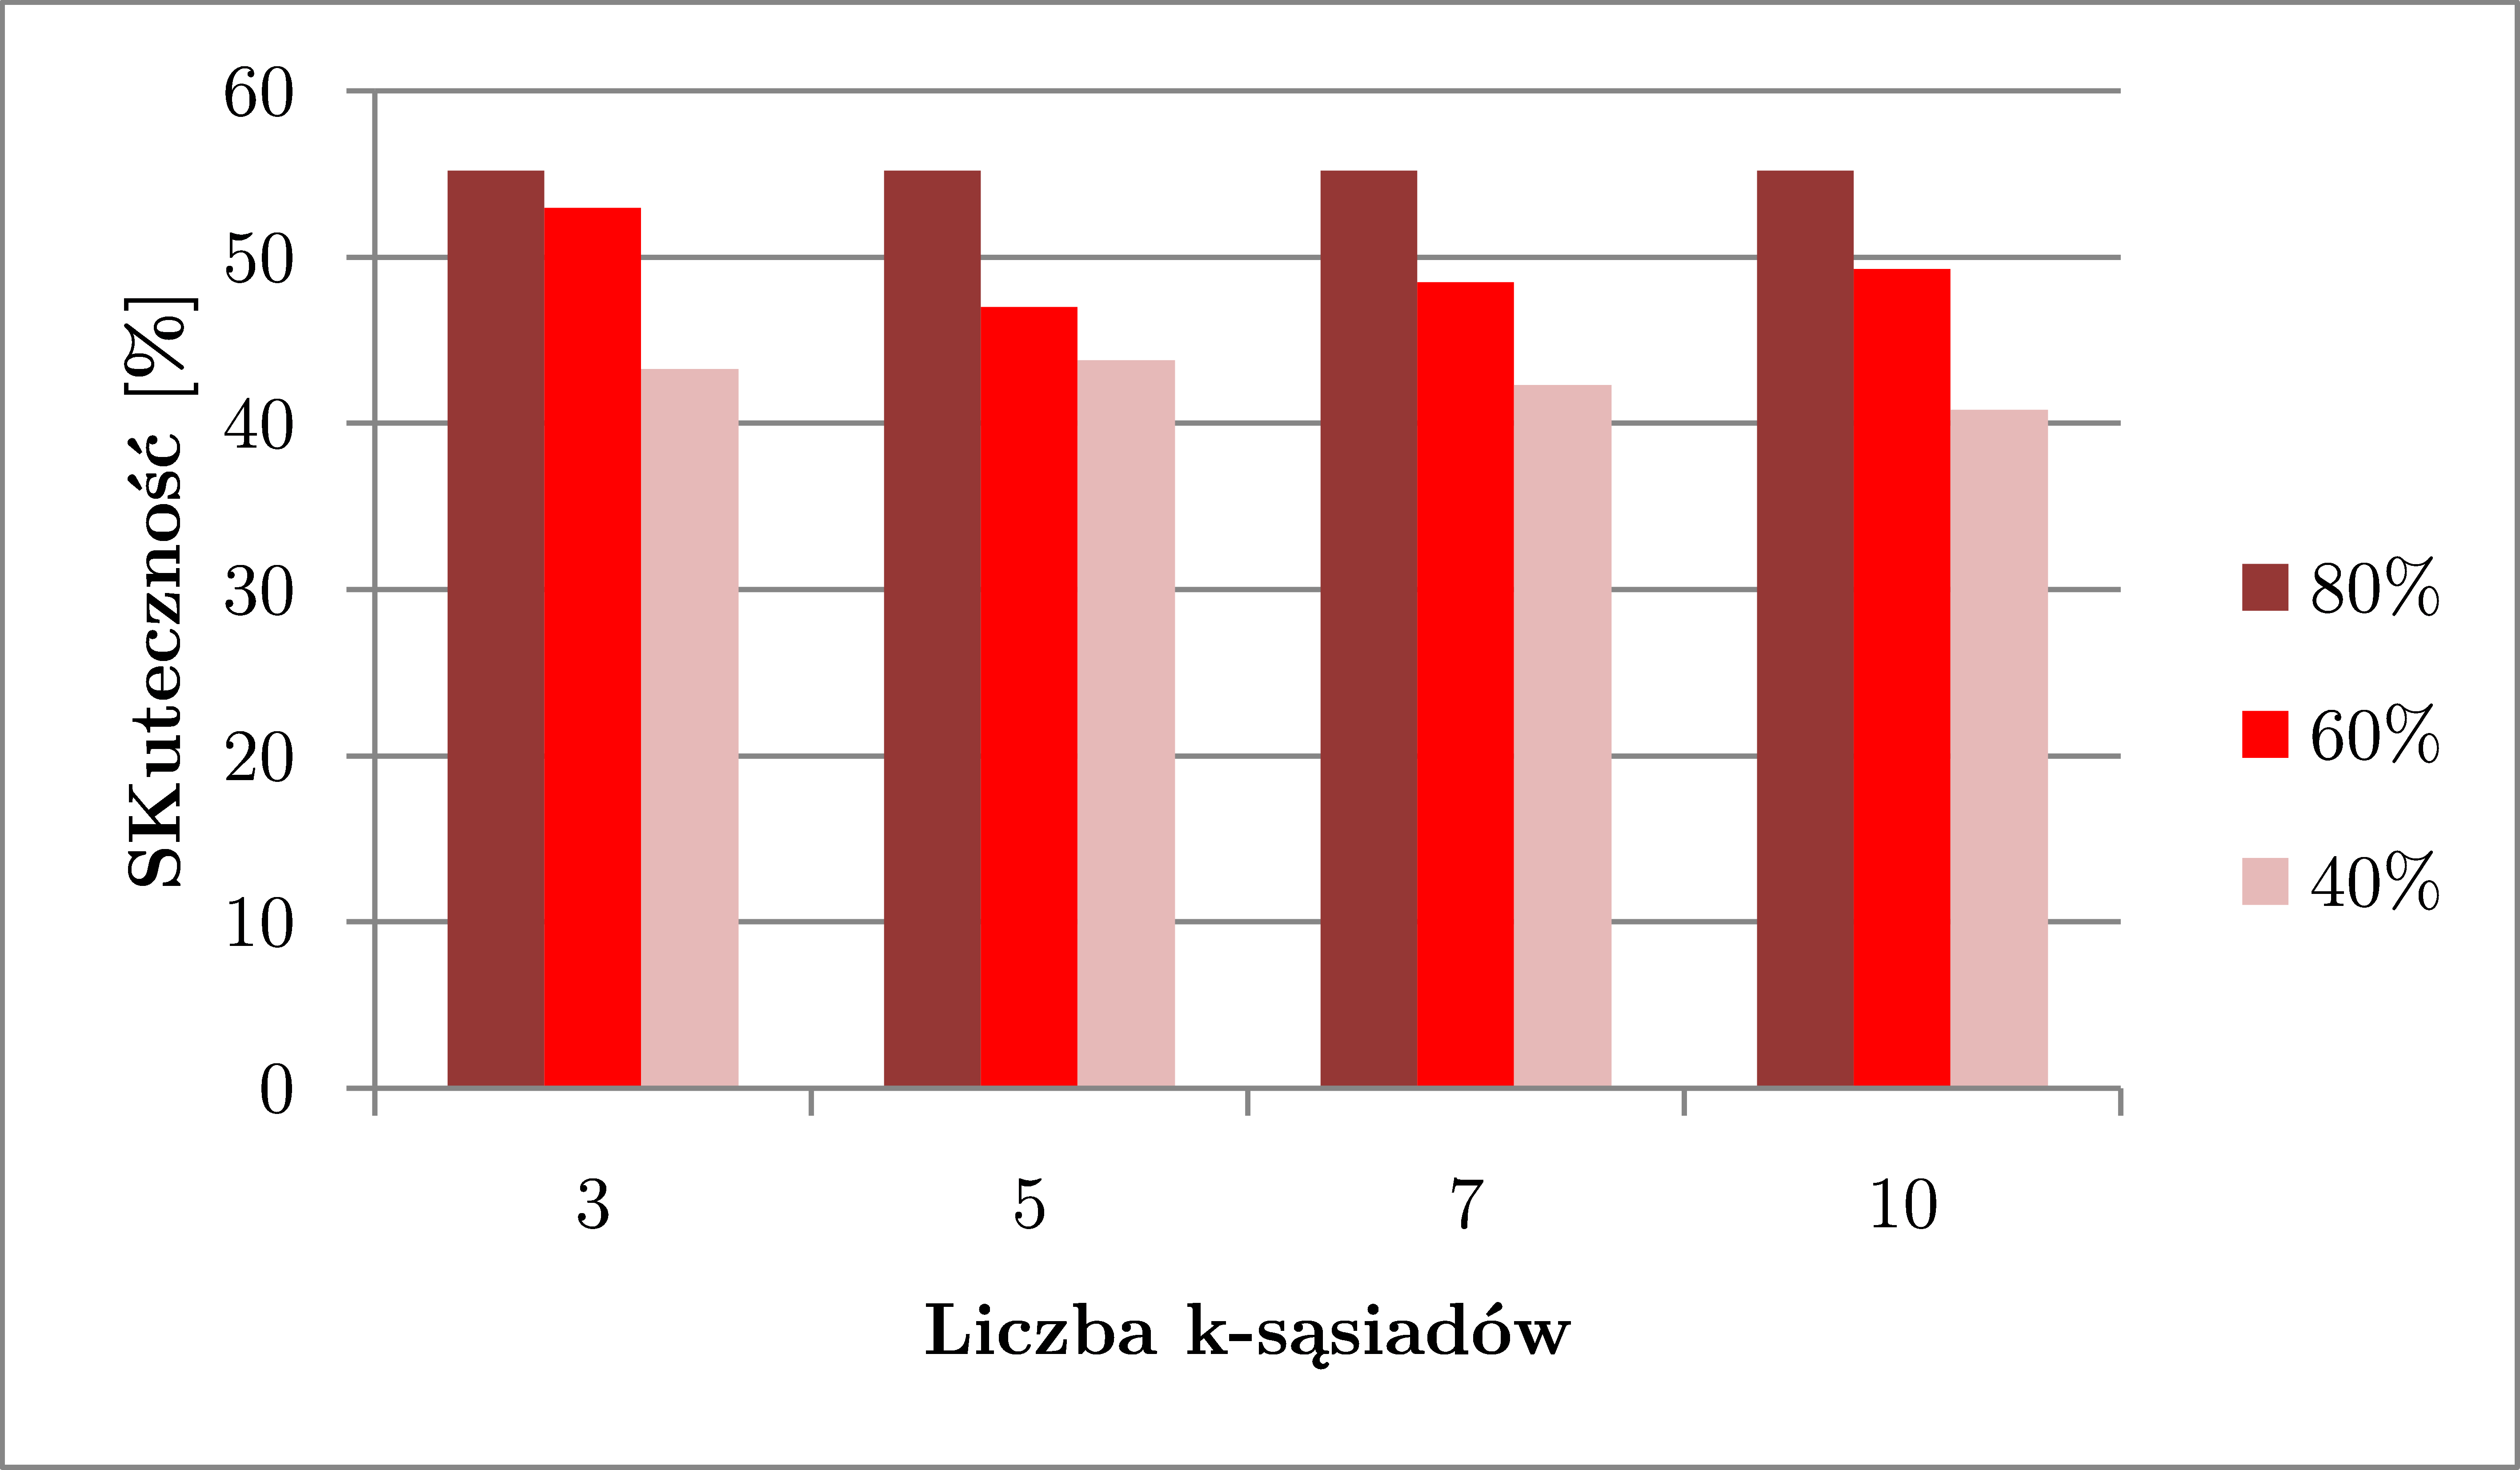
\includegraphics[width=0.9\textwidth]{{Rysunki/OWN-80-60-40-topics.png}}
	\caption{Dane z Tabel 13-15 dla kategorii topics}
\end{figure}

\begin{figure}[H]
	\centering
	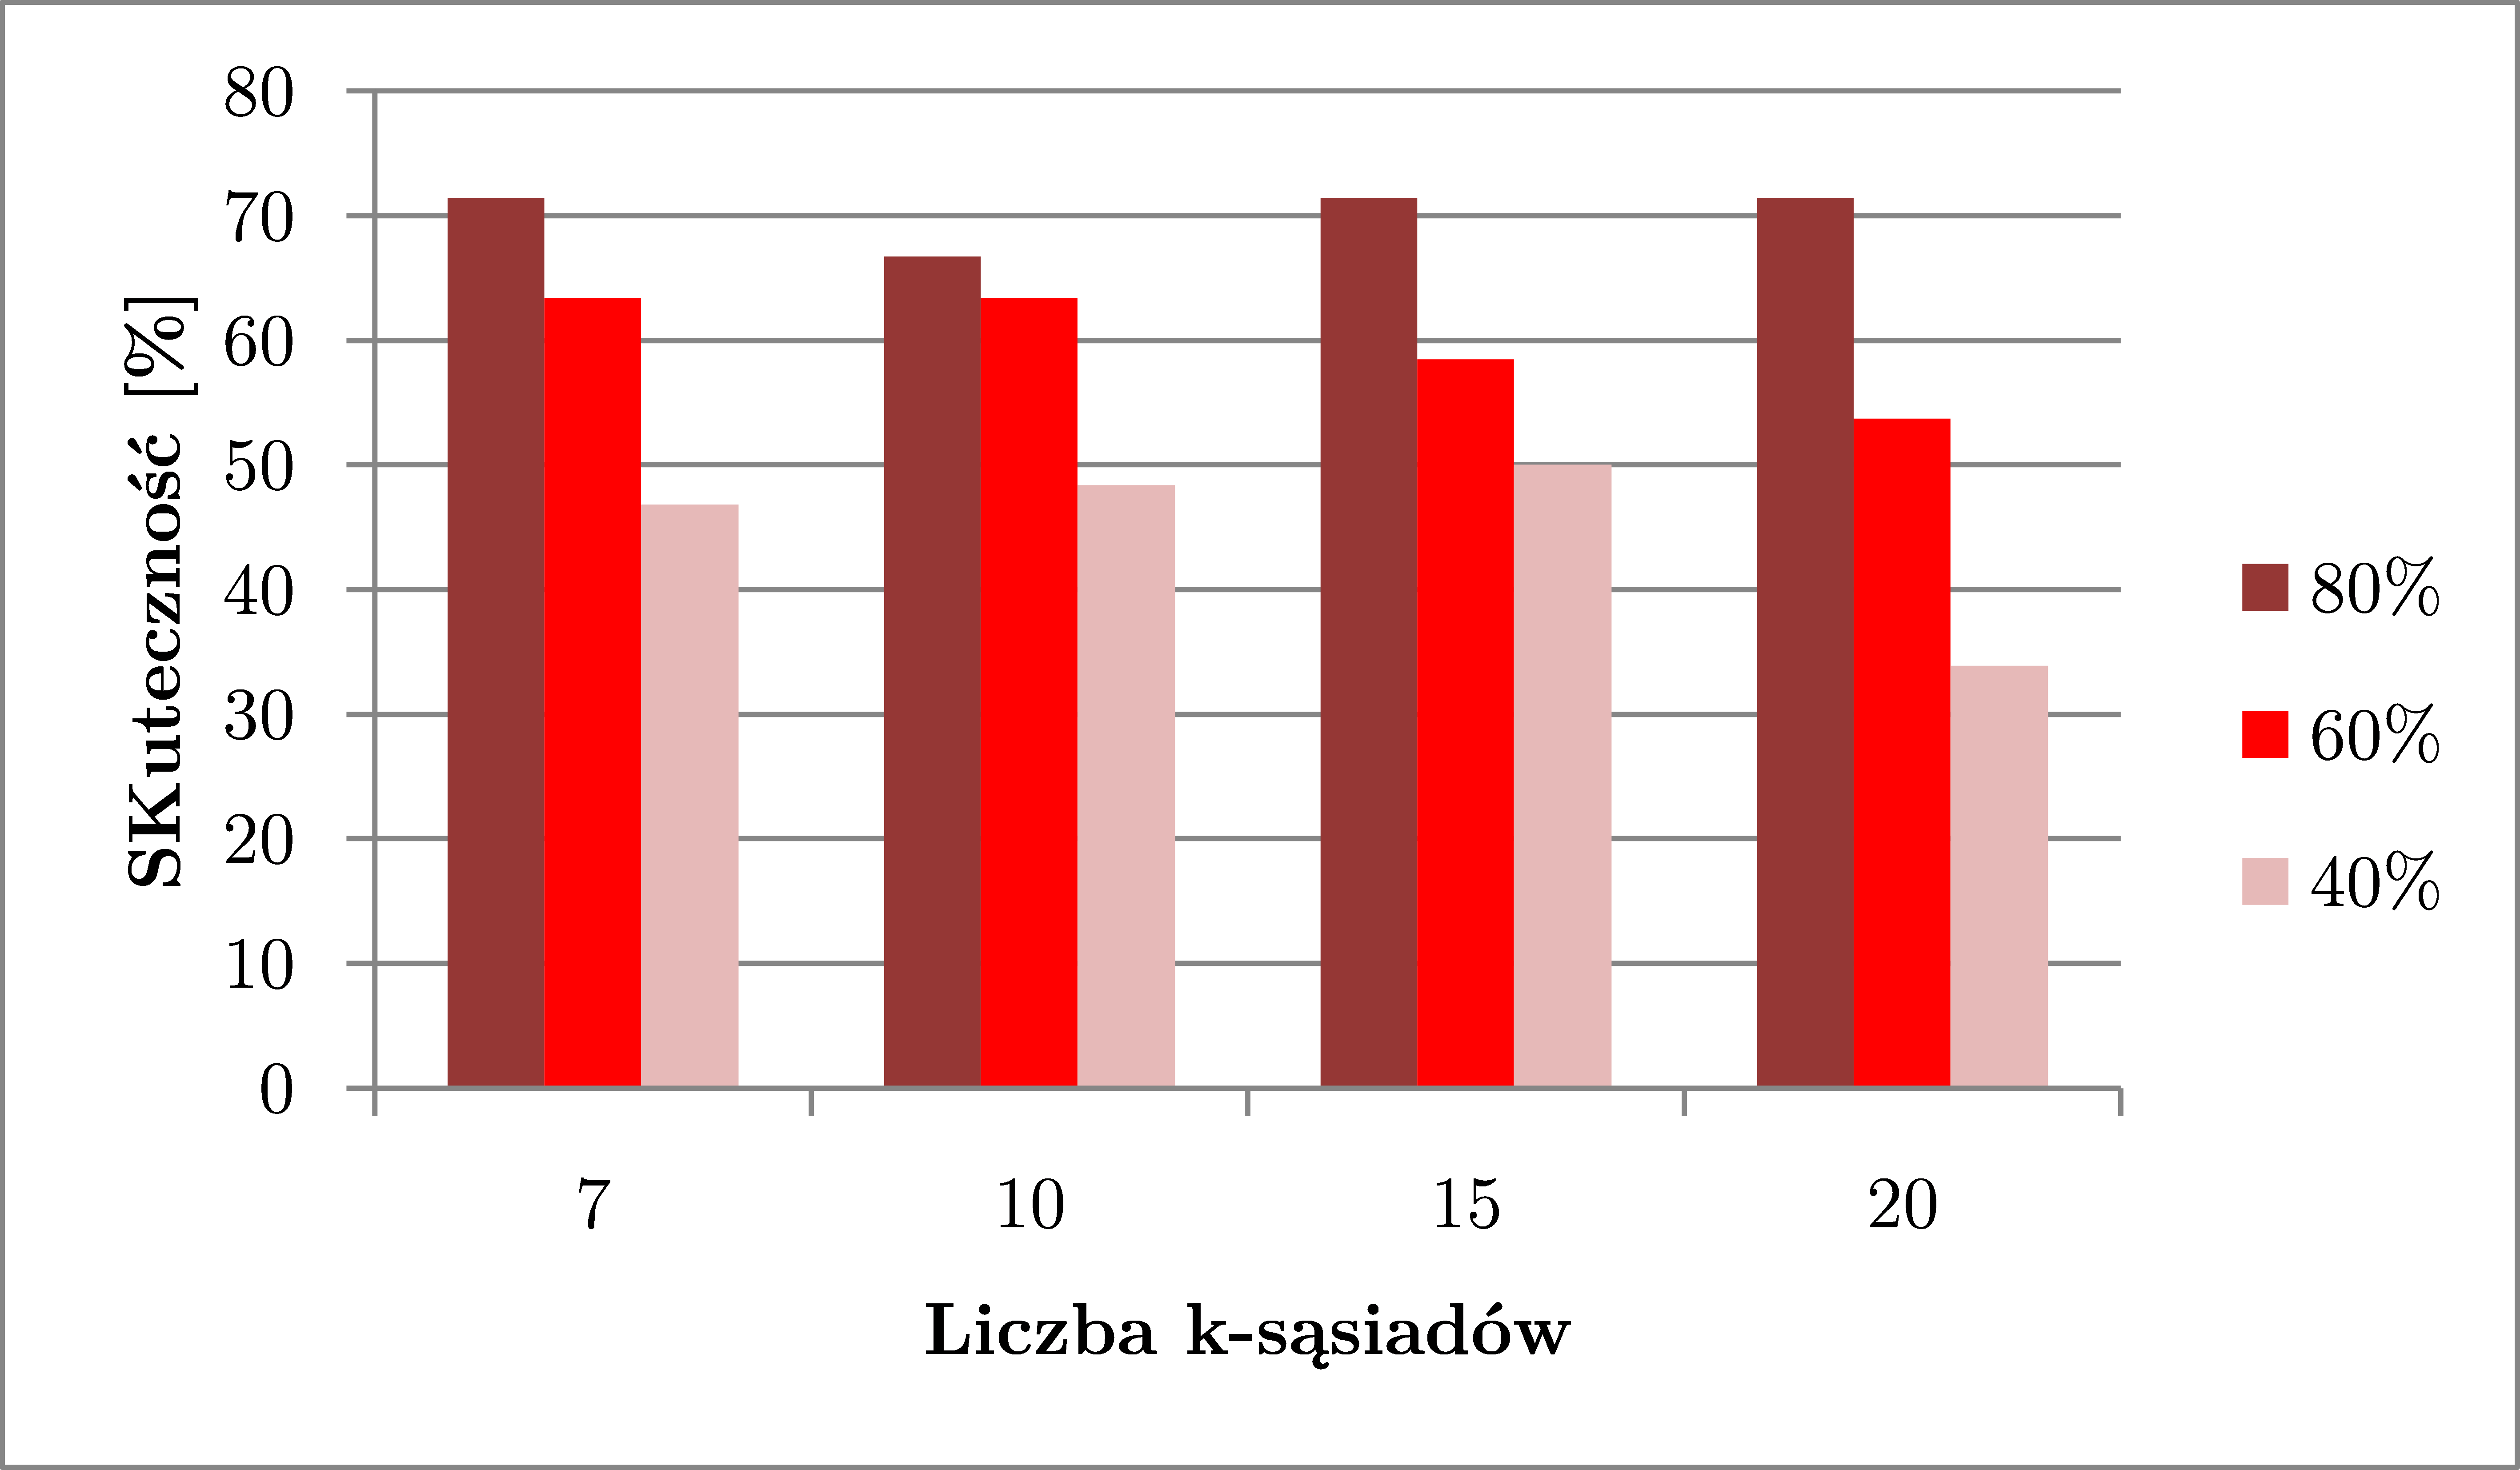
\includegraphics[width=0.9\textwidth]{{Rysunki/OWN-80-60-40-authors.png}}
	\caption{Dane z Tabel 13-15 dla kategorii authors (własne teksty)}
\end{figure}

\subsection{Wpływ konkretnych cech na klasyfikację}

W tabelach z wynikami będziemy używać następujących skrótów:
\begin{description}
	\item [$c_{1})$] Liczba słów,
	\item [$c_{2})$] Liczba słów, których długość nie przekracza 3 znaków,
	\item [$c_{3})$] Liczba słów, których długość zawiera się w zakresie 4-7 znaków,
	\item [$c_{4})$] Liczba słów, których długość przekracza 8 znaków,
	\item [$c_{5})$] Liczba unikalnych słów,
	\item [$c_{6})$] Liczba słów napisanych wielką literą,
	\item [$c_{7})$] liczba słów rozpoczynających się wielką literą. 
\end{description}

\section{Dyskusja}

\subsection{Kategoria places oraz topic}
Po przeprowadzonych badaniach jesteśmy w stanie zauważyć, iż metryka uliczna charakteryzuje się największą skutecznością w przypadku pierwszego, jak i drugiego sposobu ekstrakcji cech. Niewiele mniejszą skuteczność wykazuje metryka Euklidesowa. Z kolei, najmniejszą skuteczność reprezentuje metryka Czebyszewa. W przeciwieństwo do dwóch pozostałych metryk, zmiana ilości k sąsiadów nie wpływała lub wpływała nieznacząco na liczbę dopasowanych dokumentów. \newline

Niska liczba liczba k-sąsiadów (od 2 do 5) zazwyczaj oraz bardzo wysoka (20) zazwyczaj negatywnie wpływały na skuteczność klasyfikacji. Optymalne wartości k w przypadku algorytmu k-NN wynosiły 10 i 15 w przypadku ekstrakcji metodą term frequency oraz 7 i 10 w przypadku ekstrakcji inverse document frequency. \newline

Dwie użyte przez nas metody ekstrakcji cech wykazują bardzo podobną skuteczność - inverse document frequency nieznacznie przewyższa term frequency. Może to wynikać z faktu, iż IDF przeszukuje wszystkie dokumenty, a TF tylko jeden.  \newline

Skuteczność klasyfikacji była znacznie wyższa dla kategorii places. Zazwyczaj oscylowała wokół 80%. Z kolei, dla kategorii topics w okolicach 50%. 

\subsection{Kategoria authors (własne teksty)}
Wyniki klasyfikacji dla własnych tekstów są wyraźnie gorsze niż dla artykułów Reutersa. Przypisanie autora do tekstu jego utworu jest dużo cięższym zadaniem, z którym nasz program sobie nie radzi tak dobrze. Poza małym zbiorem danych problemem jest dużo mniejsze powiązanie słów z danym autorem - mimo wybrania tekstów z jednej płyty, teksty nie były aż tak podobne tematycznie, by wyniki klasyfikacji były zadowalające.

Metryka Euklidesowa wykazuje największą skuteczność w przypadku pierwszego, jak i drugiego sposobu ekstrakcji cech. Metryka uliczna osiąga nieznacznie niższą skuteczność w porównaniu do metryki Euklidesowej. Wyniki osiągane przez metrykę Czebyszewa nie były dla nas zaskakujące. Metryka ta, tak samo jak w przypadku klasyfikacji kategorii places oraz topics, poradziła sobie najgorzej. Również nie widzimy wyraźnego wpływu liczby k sąsiadów na osiąganą skuteczność. \newline

W obu wybranych przez nas metodach ekstrakcji cech zauważyliśmy, iż wraz ze wzrostem liczby k sąsiadów, do pewnego momentu rośnie także osiągana skuteczność. Najwyższe wyniki pojawiają się w wypadku, gdy k jest równe 5. Najsłabsze, gdy k jest równe 7. Przy liczbie sąsiadów równej 10 i 15 skuteczność ponownie lekko wzrasta, aby przy 20 sąsiadach zacząć spadać.\newline

W klasyfikacji kategorii authors, metoda ekstrakcji term frequency wykazała się większą skutecznością, niż inverse document frequency. Jest to wyraźnie widocznie przy użyciu metryki Euklidesowej i ulicznej. W przypadku metryki Czebyszewa, wyniki okazały się identyczne. 	
	
\section{Wnioski}
\begin{itemize}
	\item Metryka Euklidesowa oraz uliczna osiągają zadowalającą skuteczność
	\item Metryka Czebyszewa nie osiąga satysfakcjonujących wyników w przypadku klasyfikacji
	\item Algorytm k-NN radzi sobie najlepiej, kiedy k nie jest zbyt niskie oraz zbyt wysokie. W zależności od doboru danych do analizowania najmniejsza ilość sąsiadów waha się od 7 do 10, zaś największa oscyluje wokół 15.
	\item Metoda k-NN przy założeniach tego zadania nie radzi sobie najlepiej z klasyfikacją piosenek do ich autorów.
\end{itemize}

	

\begin{thebibliography}{}
\bibitem{adam}
Methods for the linguistic summarization of data - aplications of fuzzy sets and their extensions, Adam Niewiadomski, Akademicka Oficyna Wydawnicza EXIT, Warszawa 2008
\bibitem{AGH}
http://home.agh.edu.pl/~horzyk/lectures/miw/KNN.pdf
\bibitem{Stop Lista}
https://github.com/hklemp/dotnet-stop-words
\bibitem{Stemizacja}
http://snowball.tartarus.org/algorithms/english/stemmer.html
\end{thebibliography}
\end{document}
